
\section{Sentiment Analysis}
\begin{figure}[htbp]
    \centering
    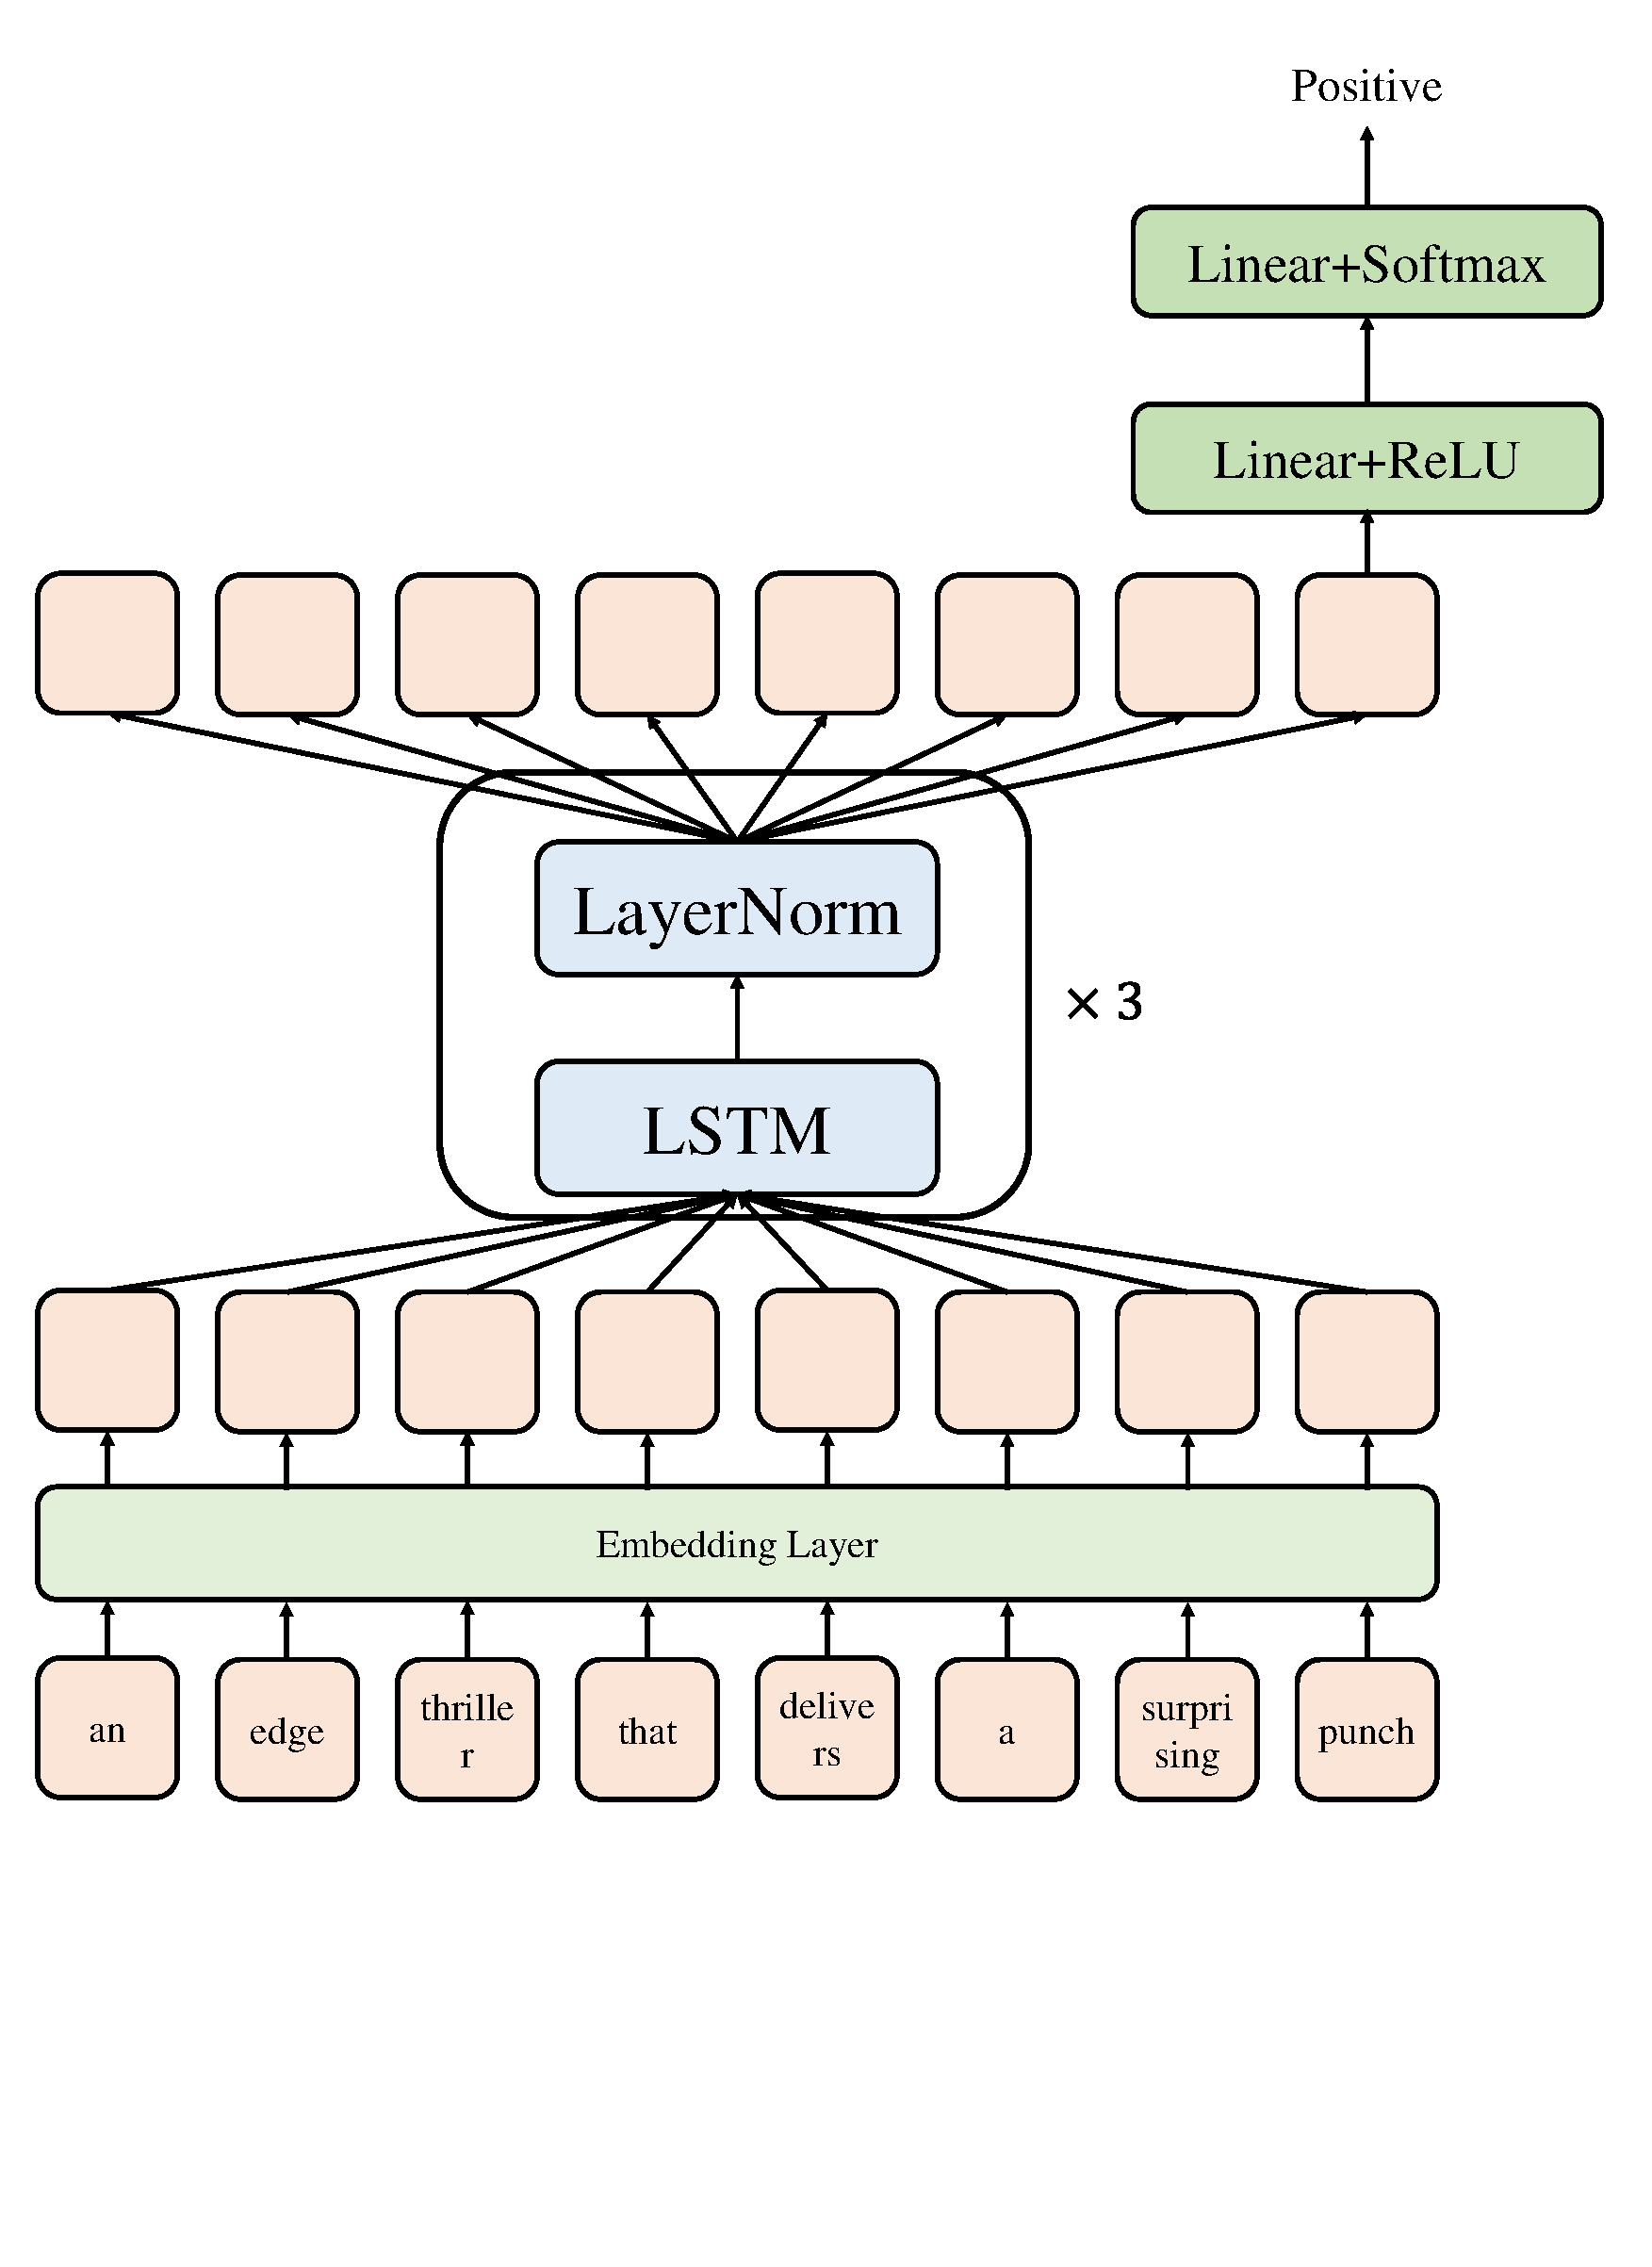
\includegraphics[width=0.5\textwidth]{lstm_model.pdf}
    \caption{Illustration of LSTM models.}
    \label{fig:lstm_model}
\end{figure}
\subsection{Model \& Hyperparameters}
The model framework is displayed at Fig.~\ref{fig:lstm_model}. I use three LSTM layers, three layer-normalization layers, two linear layers and a softmax classification layer. 
The reason for layer-normalization layer instead of batch-normalization layer is that words input are all padded with zero and not well-suitable for batch-normalization.
Because the last token stores all information from history, I use this token for classification.
The LSTM module is implemented by myself following the handout of Prof. Zhang.
In other words, I take the input sequence as the initial state of each LSTM block. And an all-zero tensor for initial hidden state.
In LSTM layer, the hidden state of each token of a sequence is incrementally updated from left to right.

\hspace*{\fill} \\
\noindent
I use 256 as the batch size and set each hidden state of LSTM layer to 512.
I ran the whole model for 105 epochs to ensure convergence.
The learning rate is set to $1\times 10^{-4}$ for stable training.
To make the model trainable, I first preprocess the dataset and precompute the longest sentence.
After that, I pad zero after other sentences that are shorter that the longest one.
I only sample 6920 sentences from the dataset and maintain the ratio of negative samples to positive samples to be nearly the same.
I split the dataset as training/validation/testing to 0.8/0.1/0.1, respectively.
Again I adopt 0.2 as the dropout rate to mitigate over-fitting.

\begin{figure}[tbp]
    \centering
    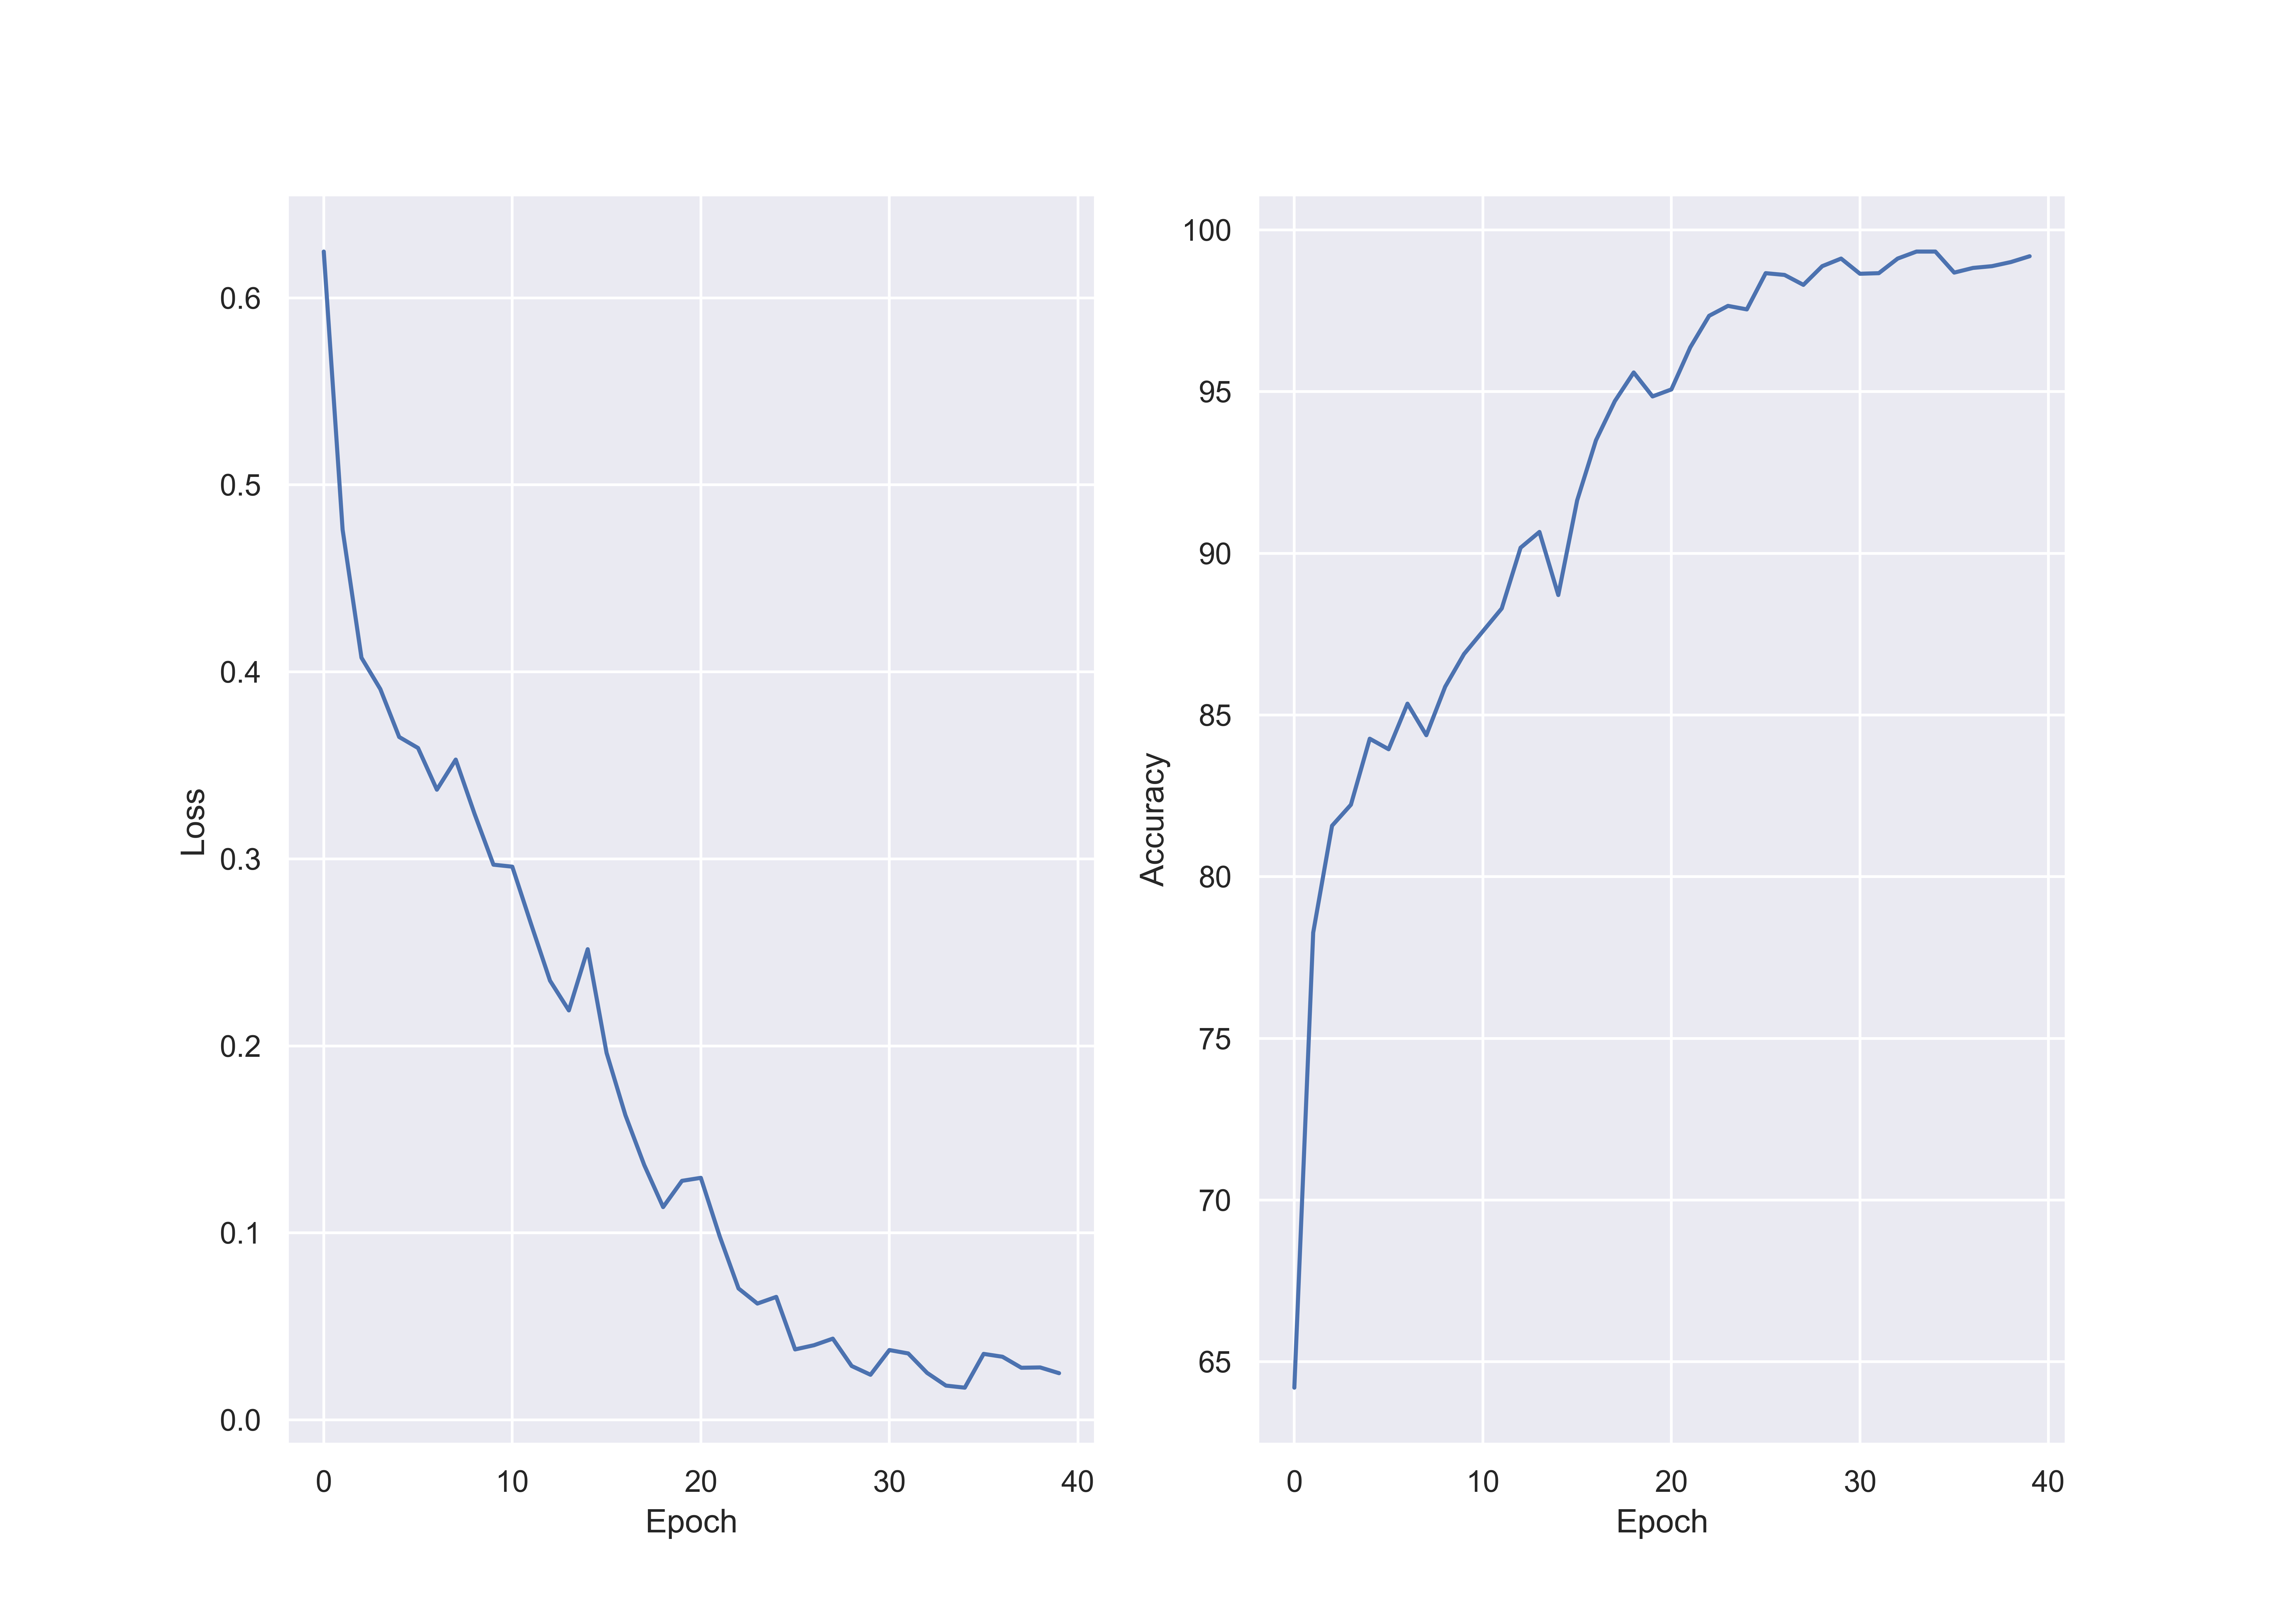
\includegraphics[width=0.9\textwidth]{../images/sst2-train-loss-acc.png}
    \caption{Change of training loss and accuracy in SST-2 dataset.}
    \label{fig:sst-train_loss}
\end{figure}
\begin{figure}[tbp]
    \centering
    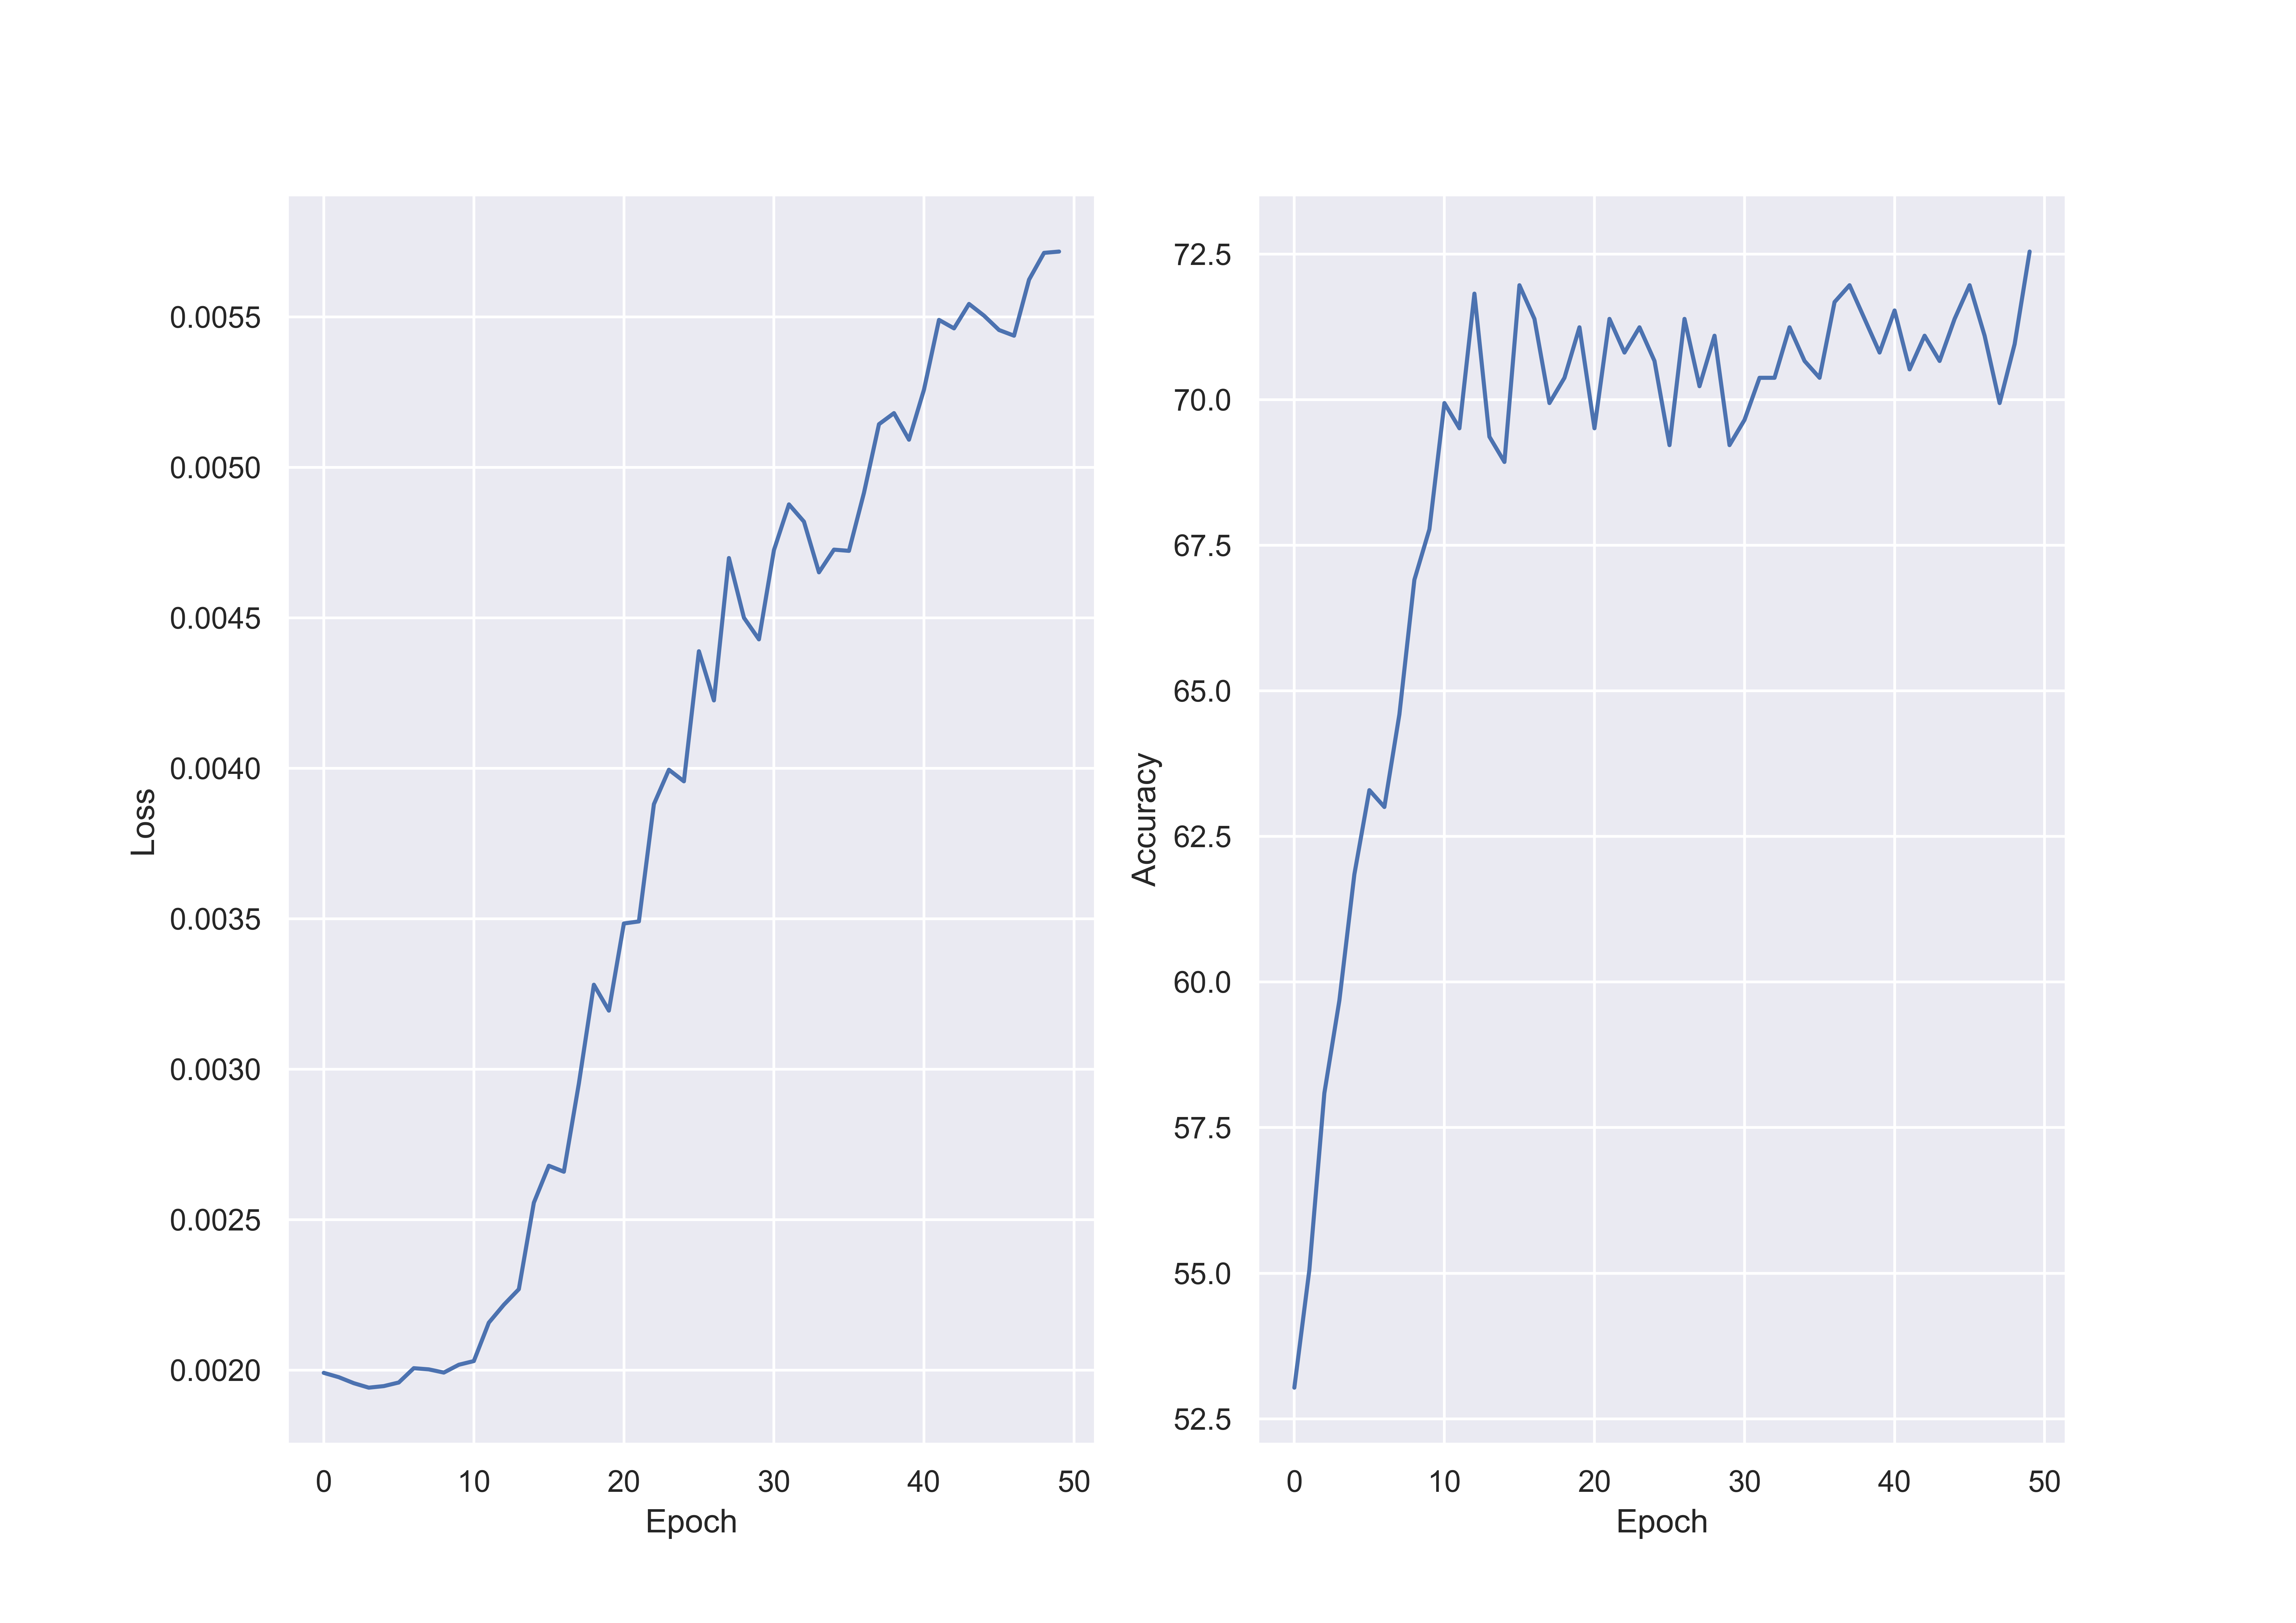
\includegraphics[width=0.9\textwidth]{../images/sst2-dev-loss-acc.png}
    \caption{Change of validation loss and accuracy in SST-2 dataset.}
    \label{fig:sst-dev_loss}
\end{figure}

\begin{figure}[htbp]
    \centering
    \begin{subfigure}
        \centering
        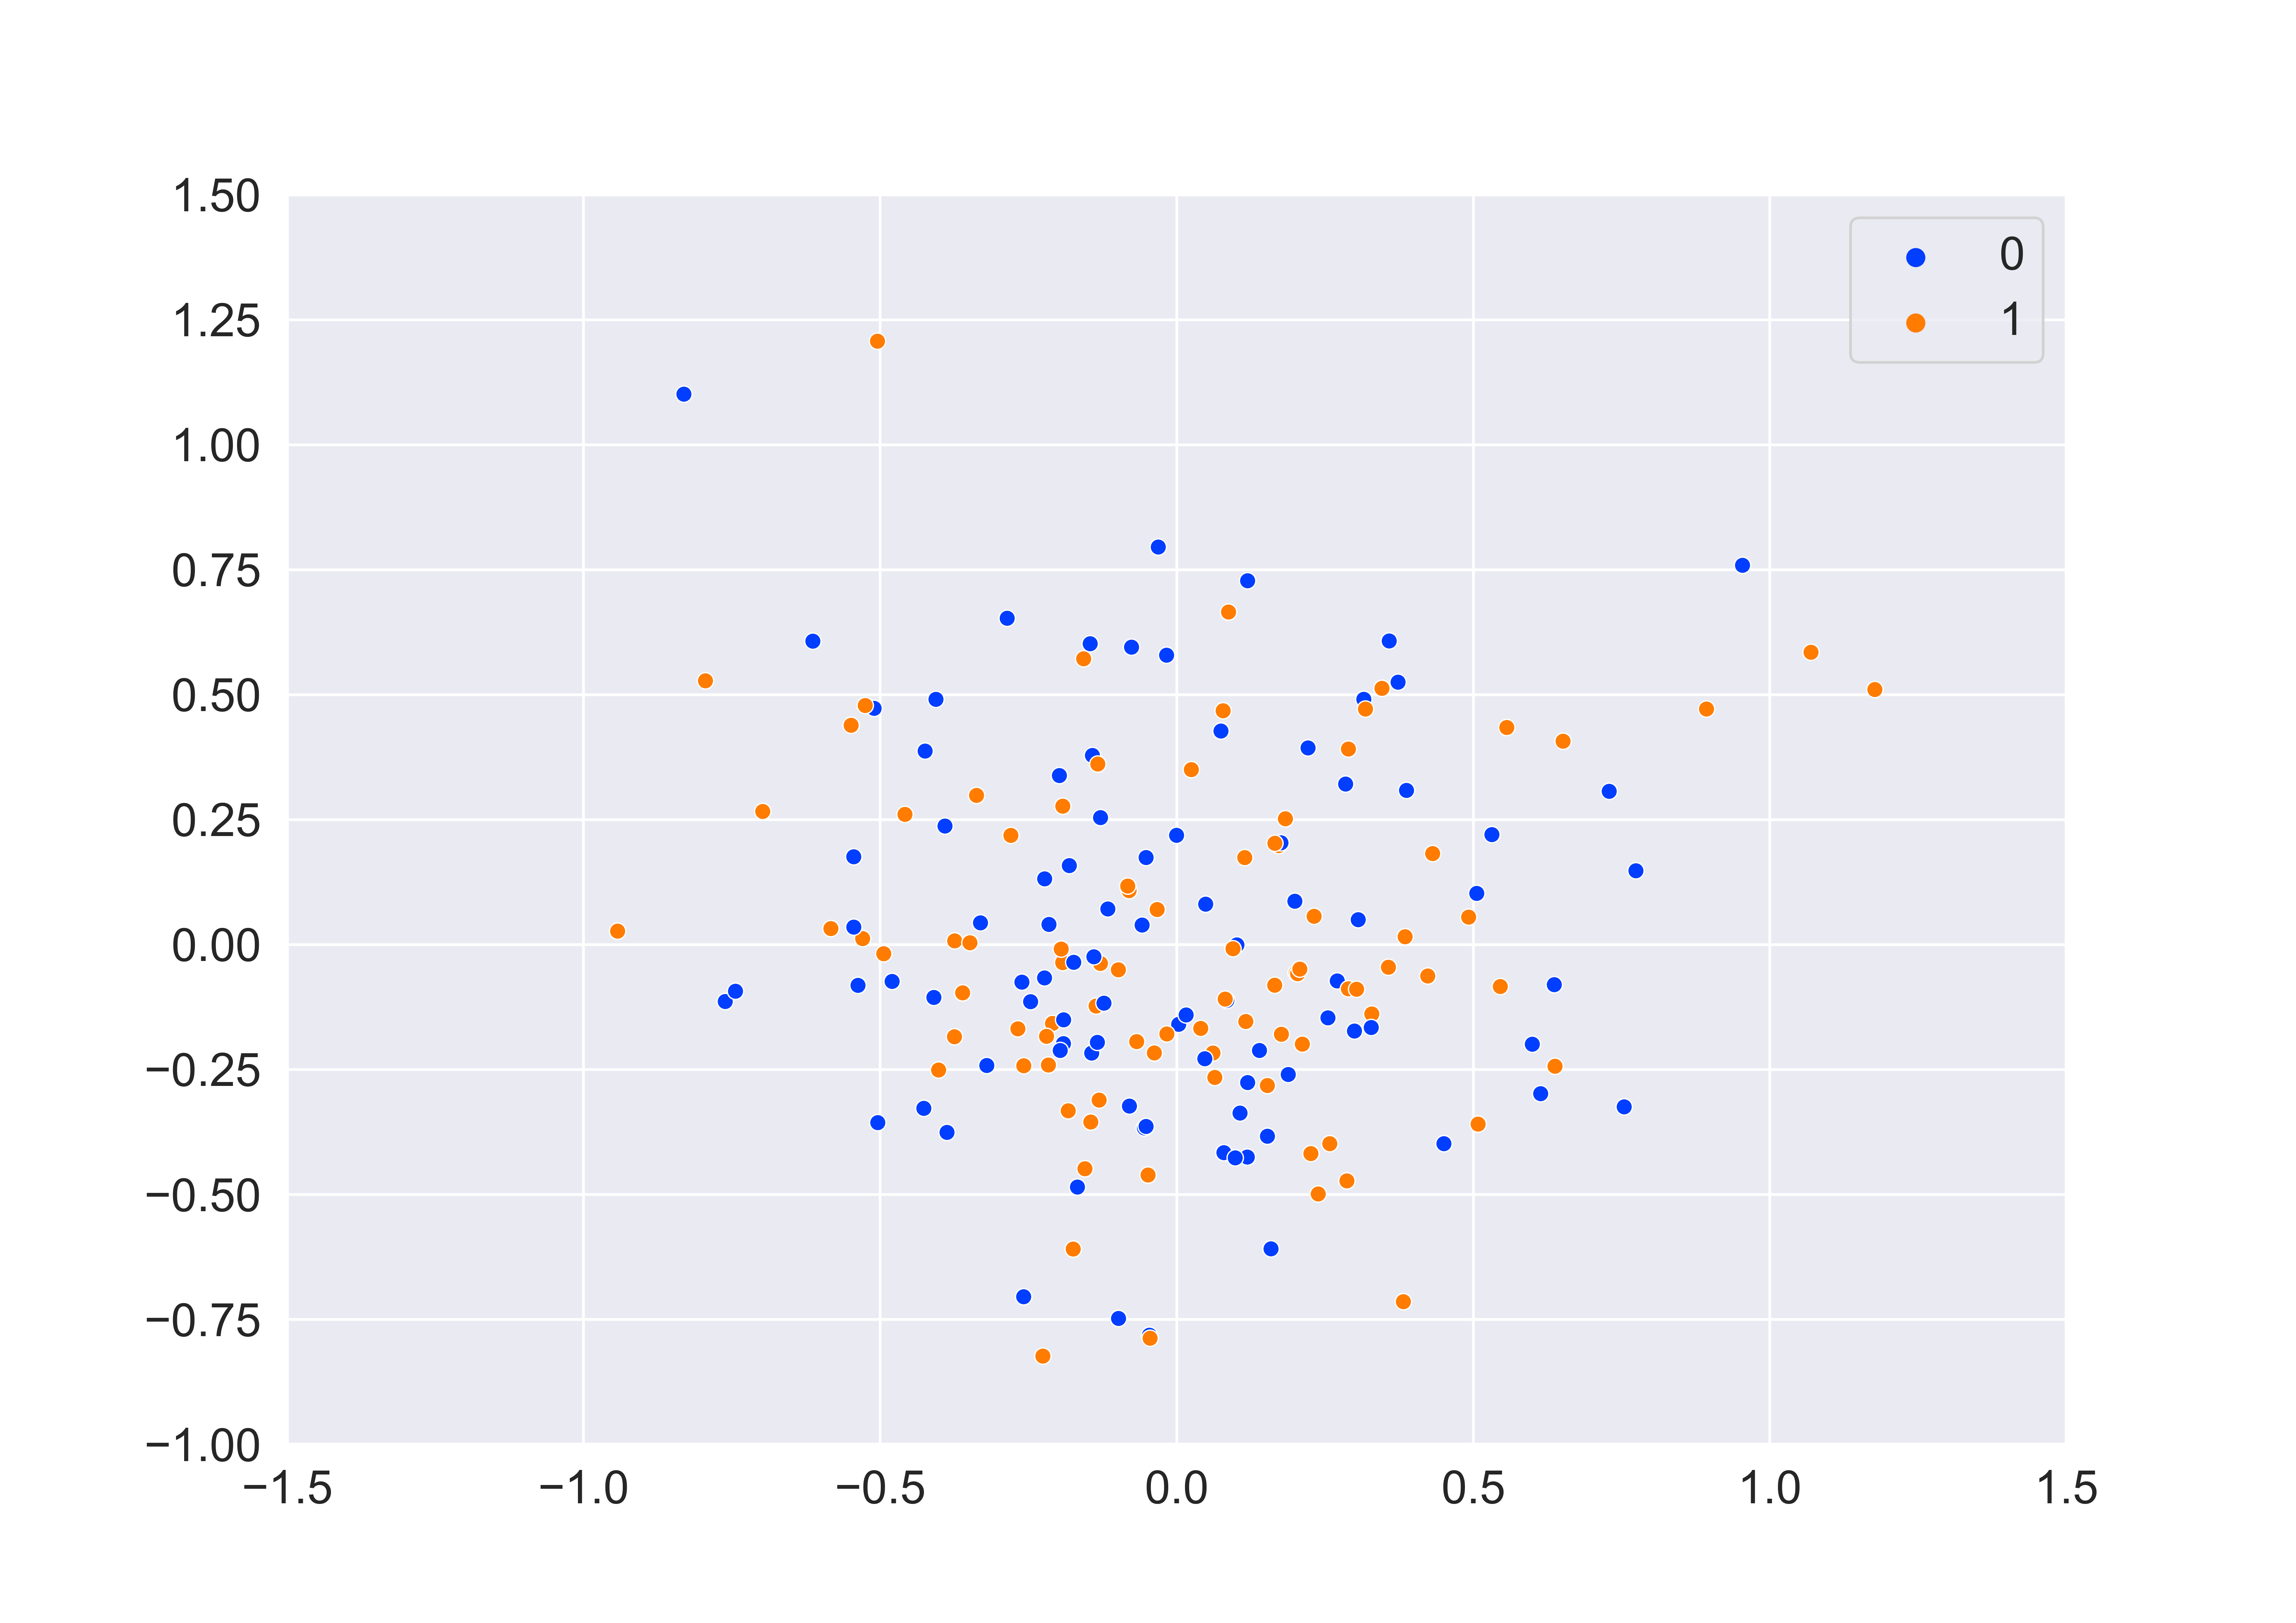
\includegraphics[width=0.45\linewidth]{../images/sst2_feature_map1_pca.png}
        % \caption{a}
        % \label{fig:mnist_tSNE_1}
    \end{subfigure}
    % \hfill 
    \begin{subfigure}
        \centering
        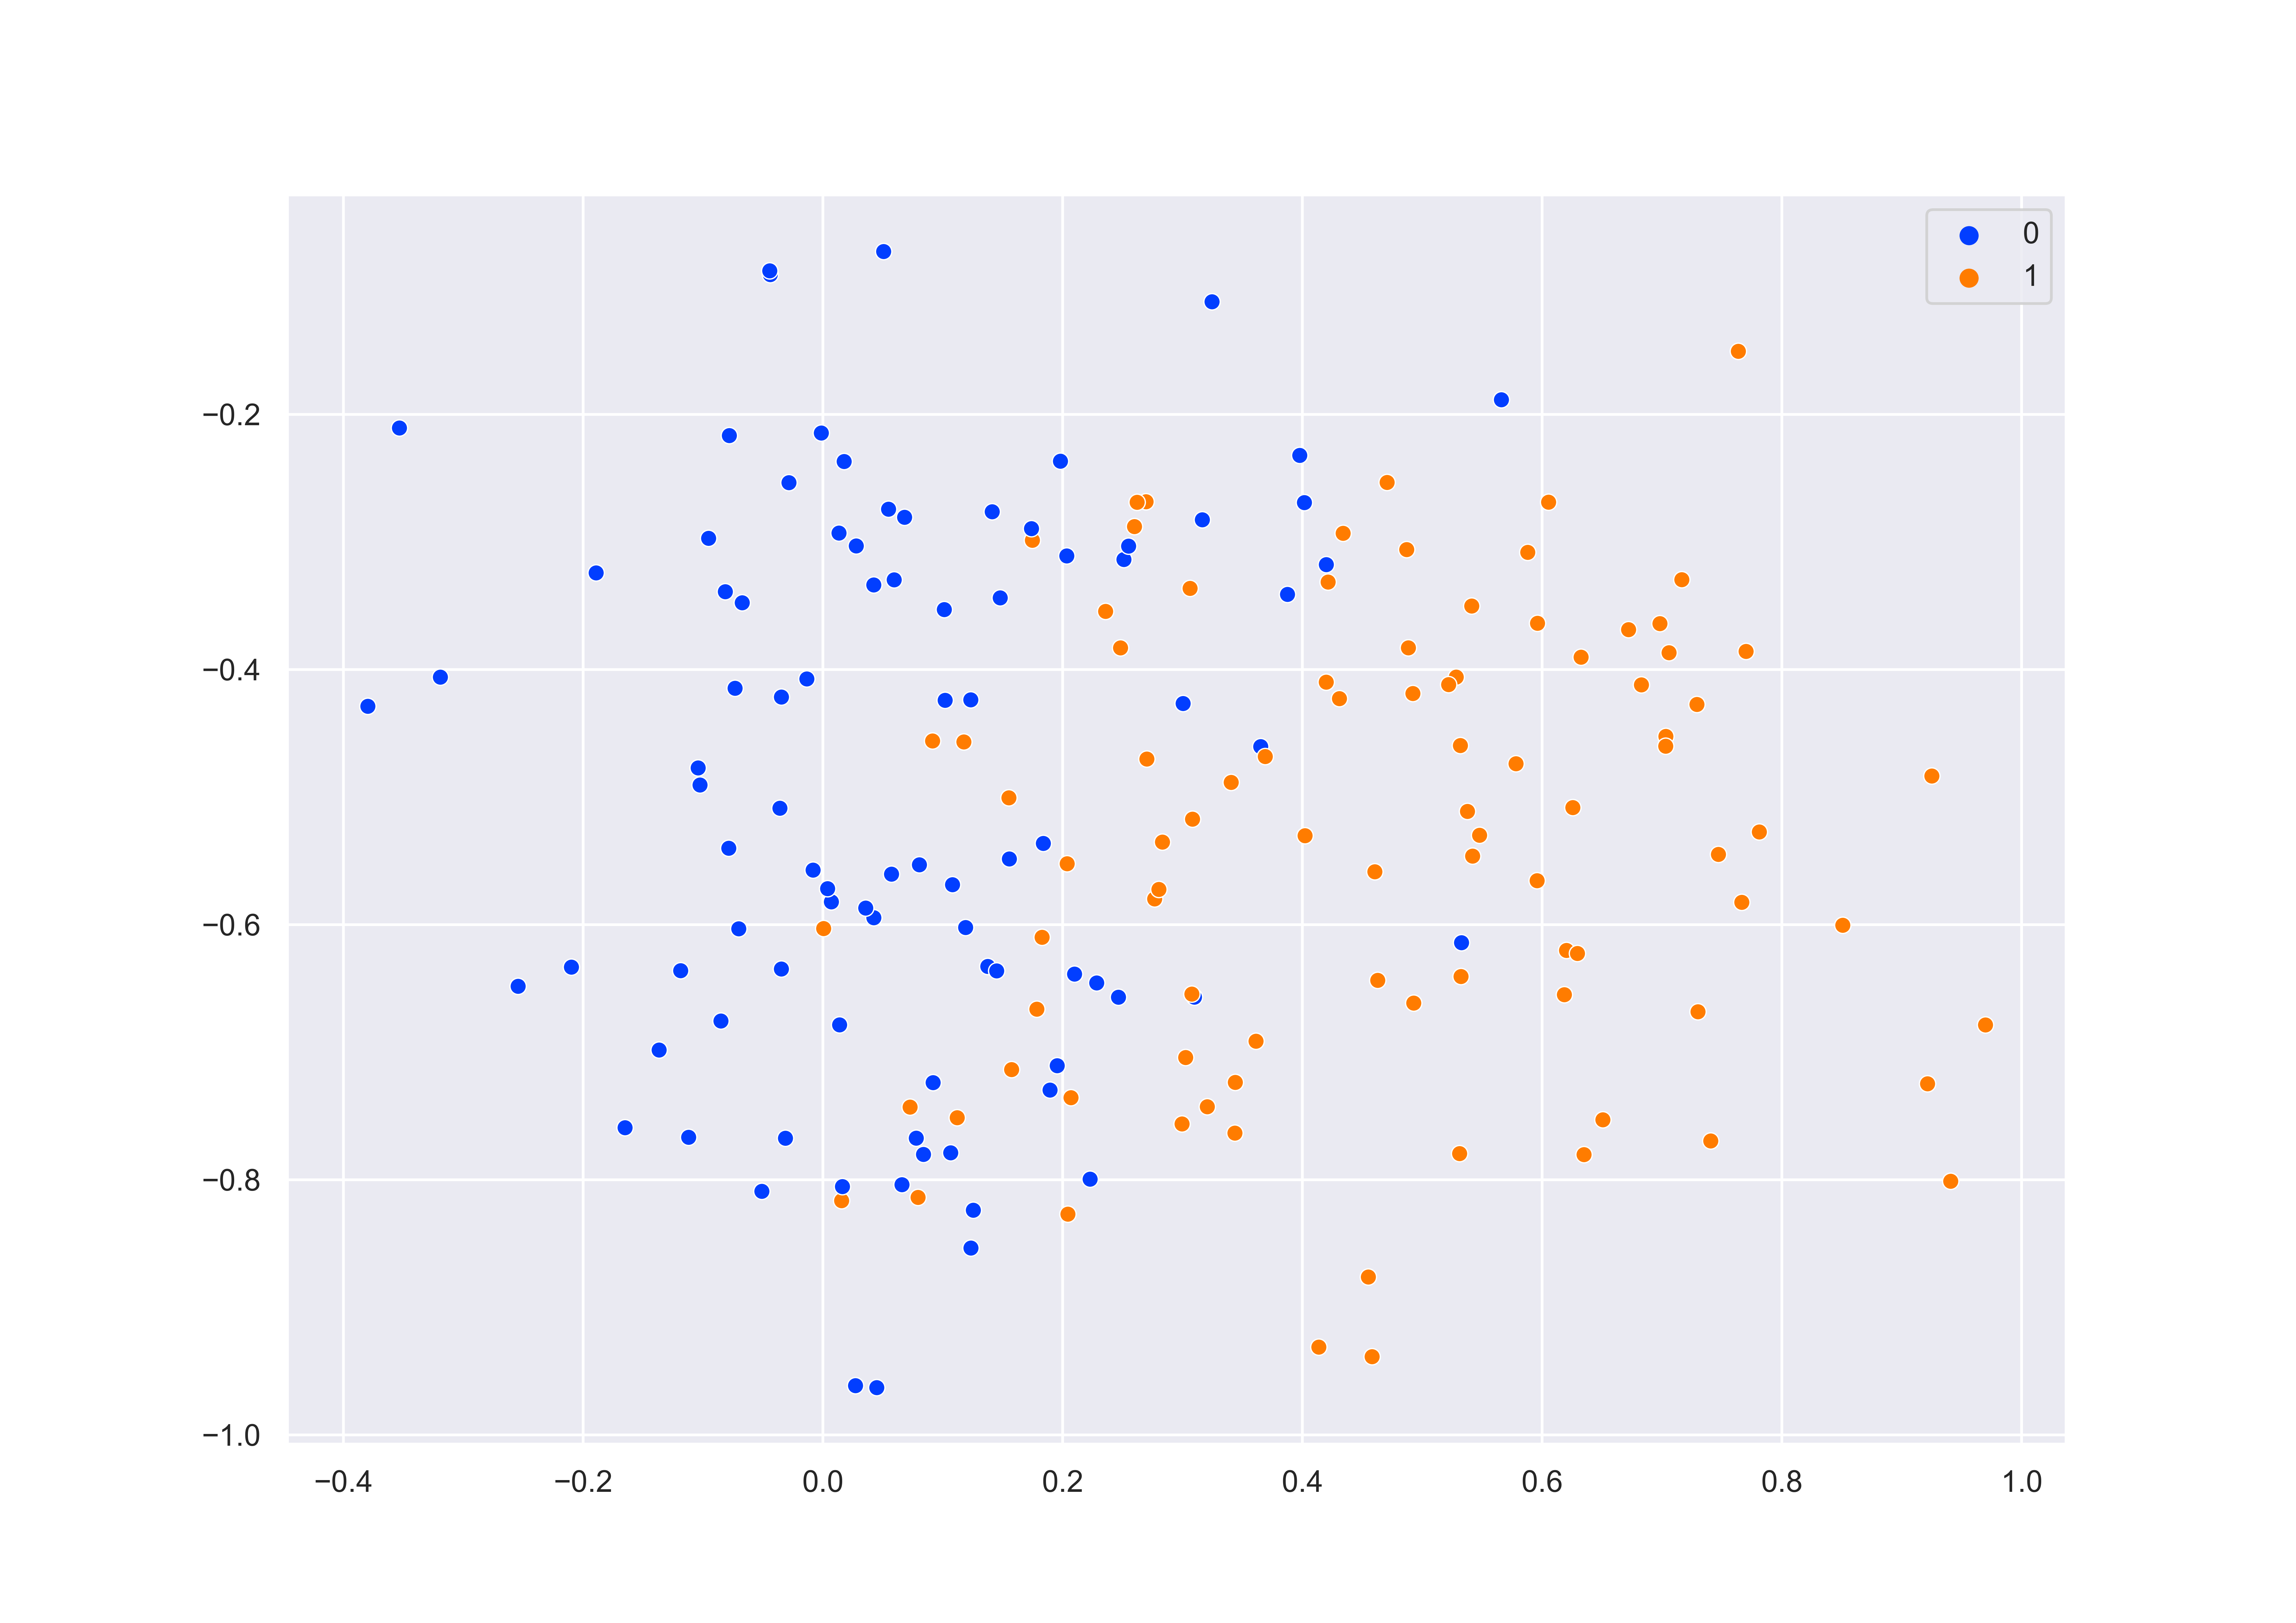
\includegraphics[width=0.45\linewidth]{../images/sst2_feature_map2_pca.png}
        % \caption{Absolute value of indivisual components of weight in ridge regression when setting $\lambda$ to 1.0.}
        % \label{fig:mnist_tSNE_2}
    \end{subfigure}
    % \hfill 
    \begin{subfigure}
        \centering
        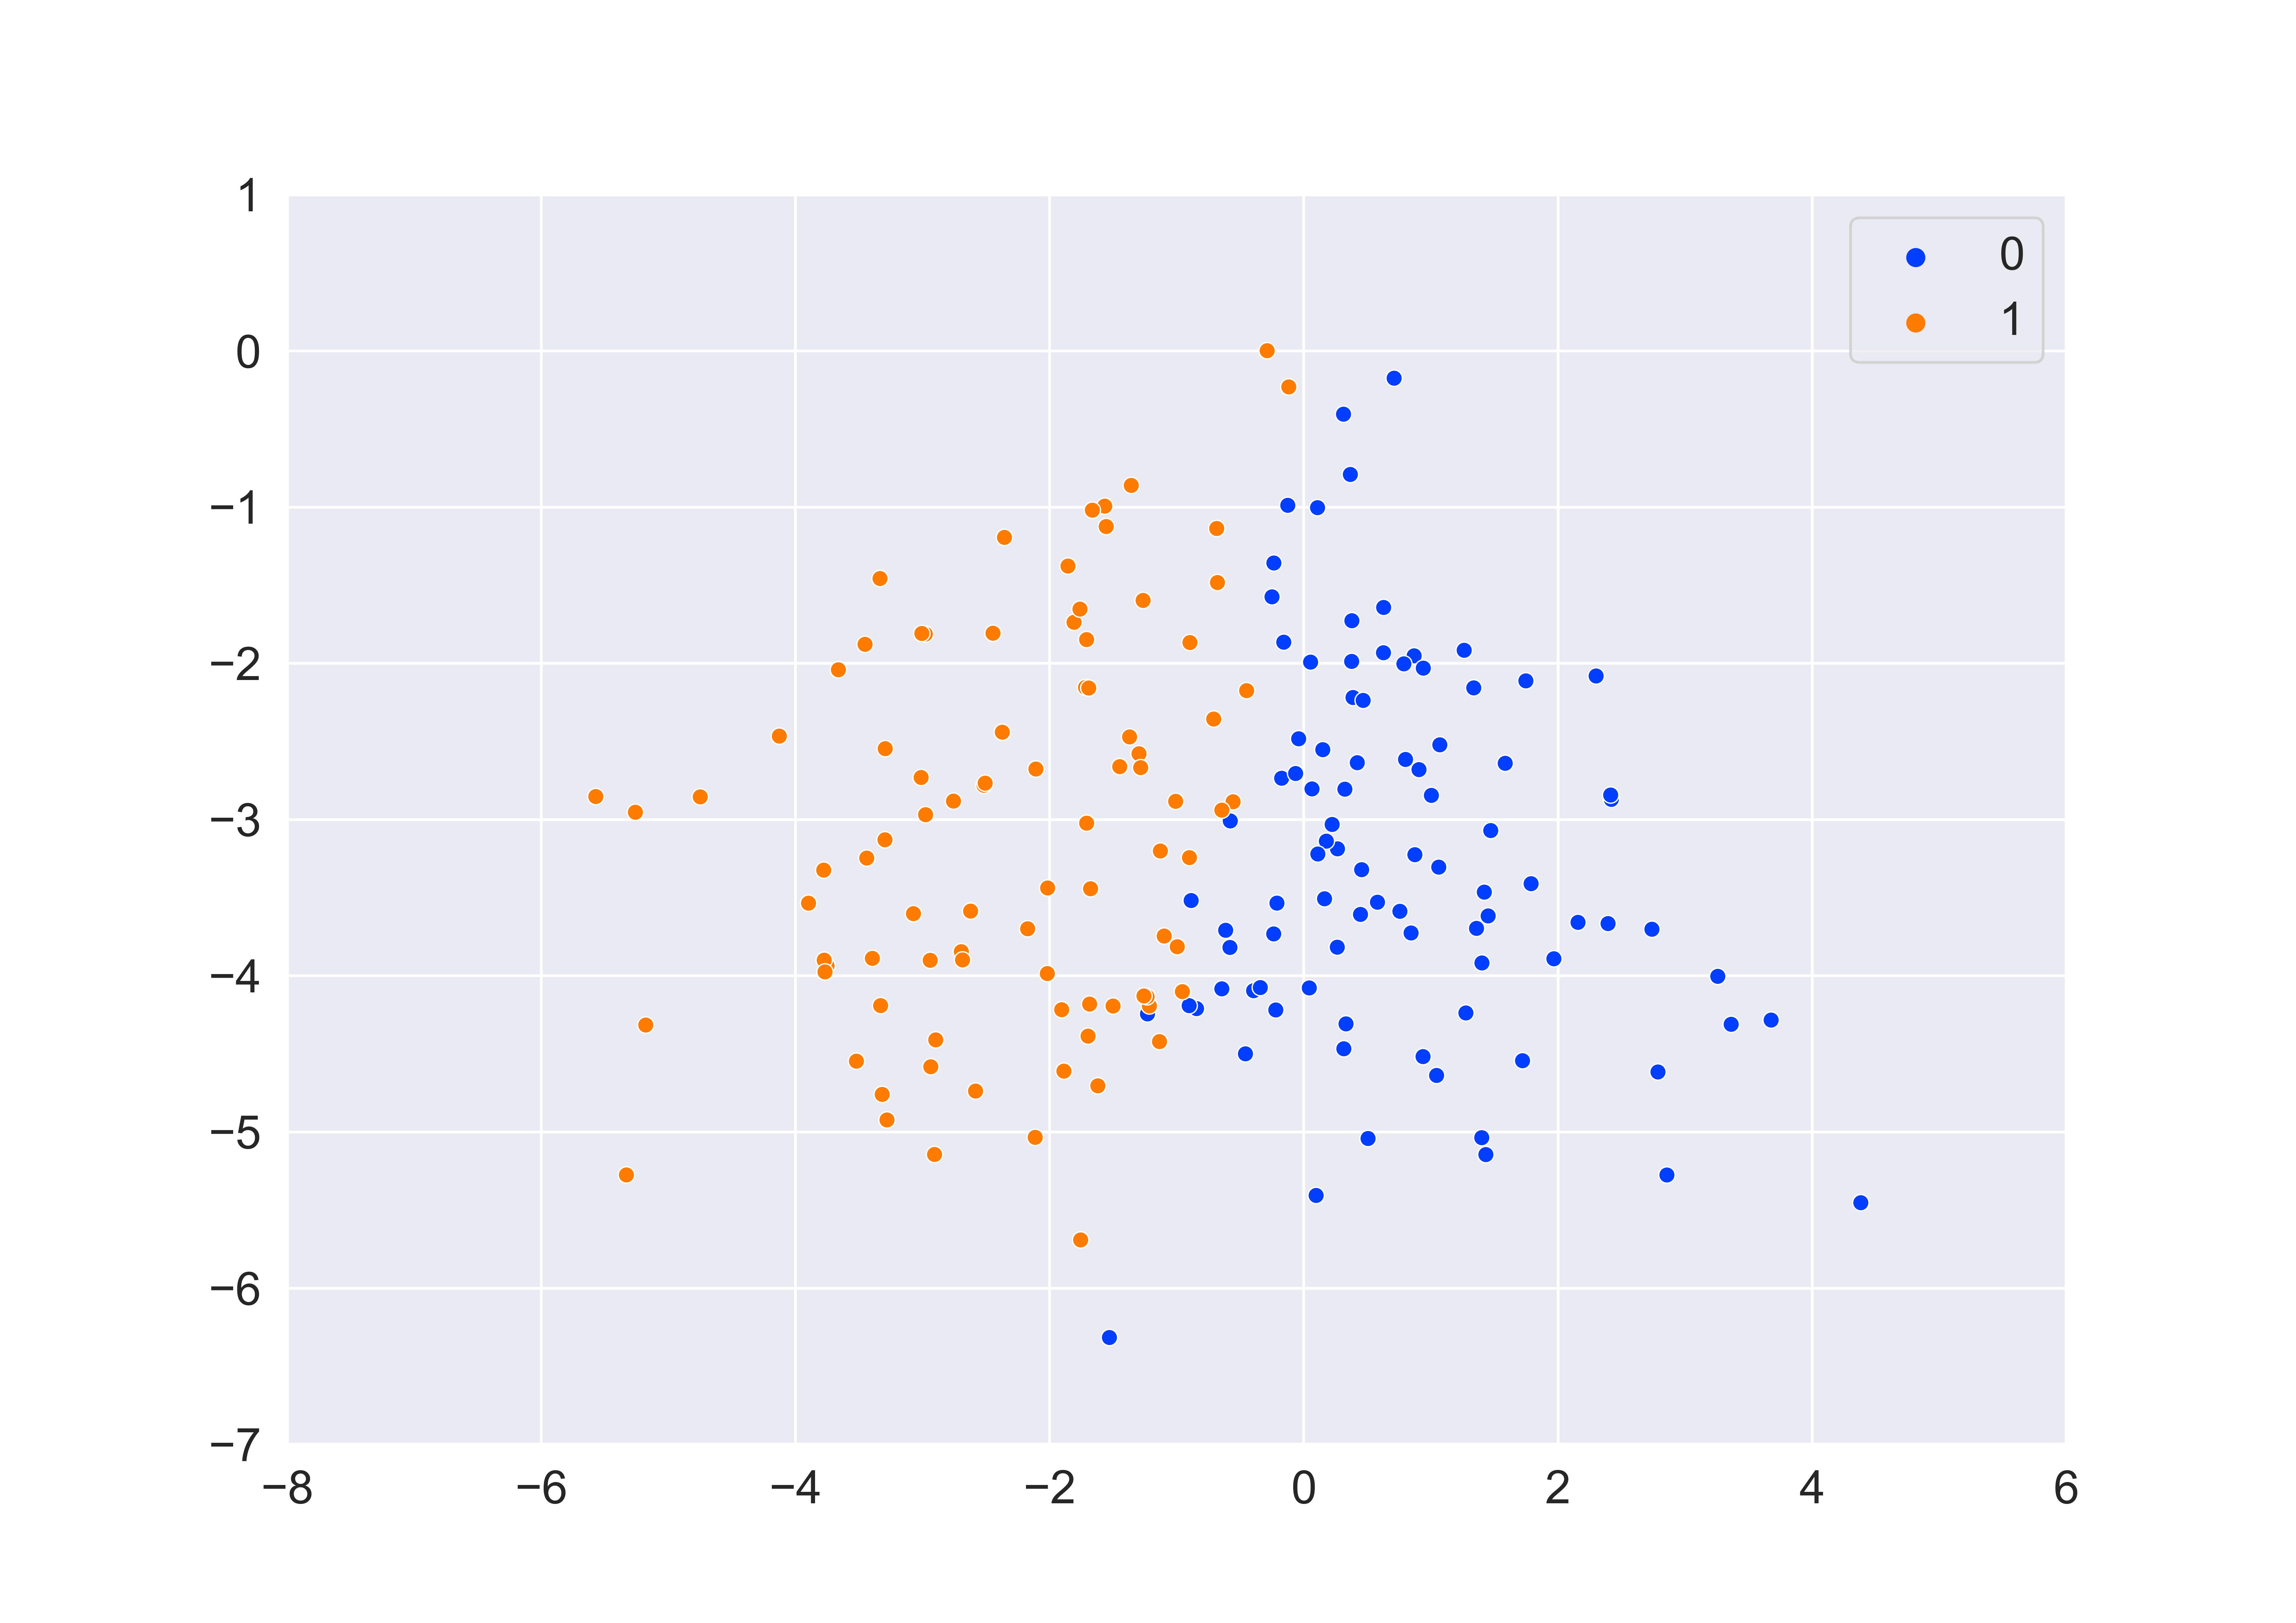
\includegraphics[width=0.45\linewidth]{../images/sst2_feature_map3_pca.png}
        % \caption{Absolute value of indivisual components of weight in ridge regression when setting $\lambda$ to 1.5.}
        % \label{fig:mnist_tSNE_3}
    \end{subfigure}
    \begin{subfigure}
        \centering
        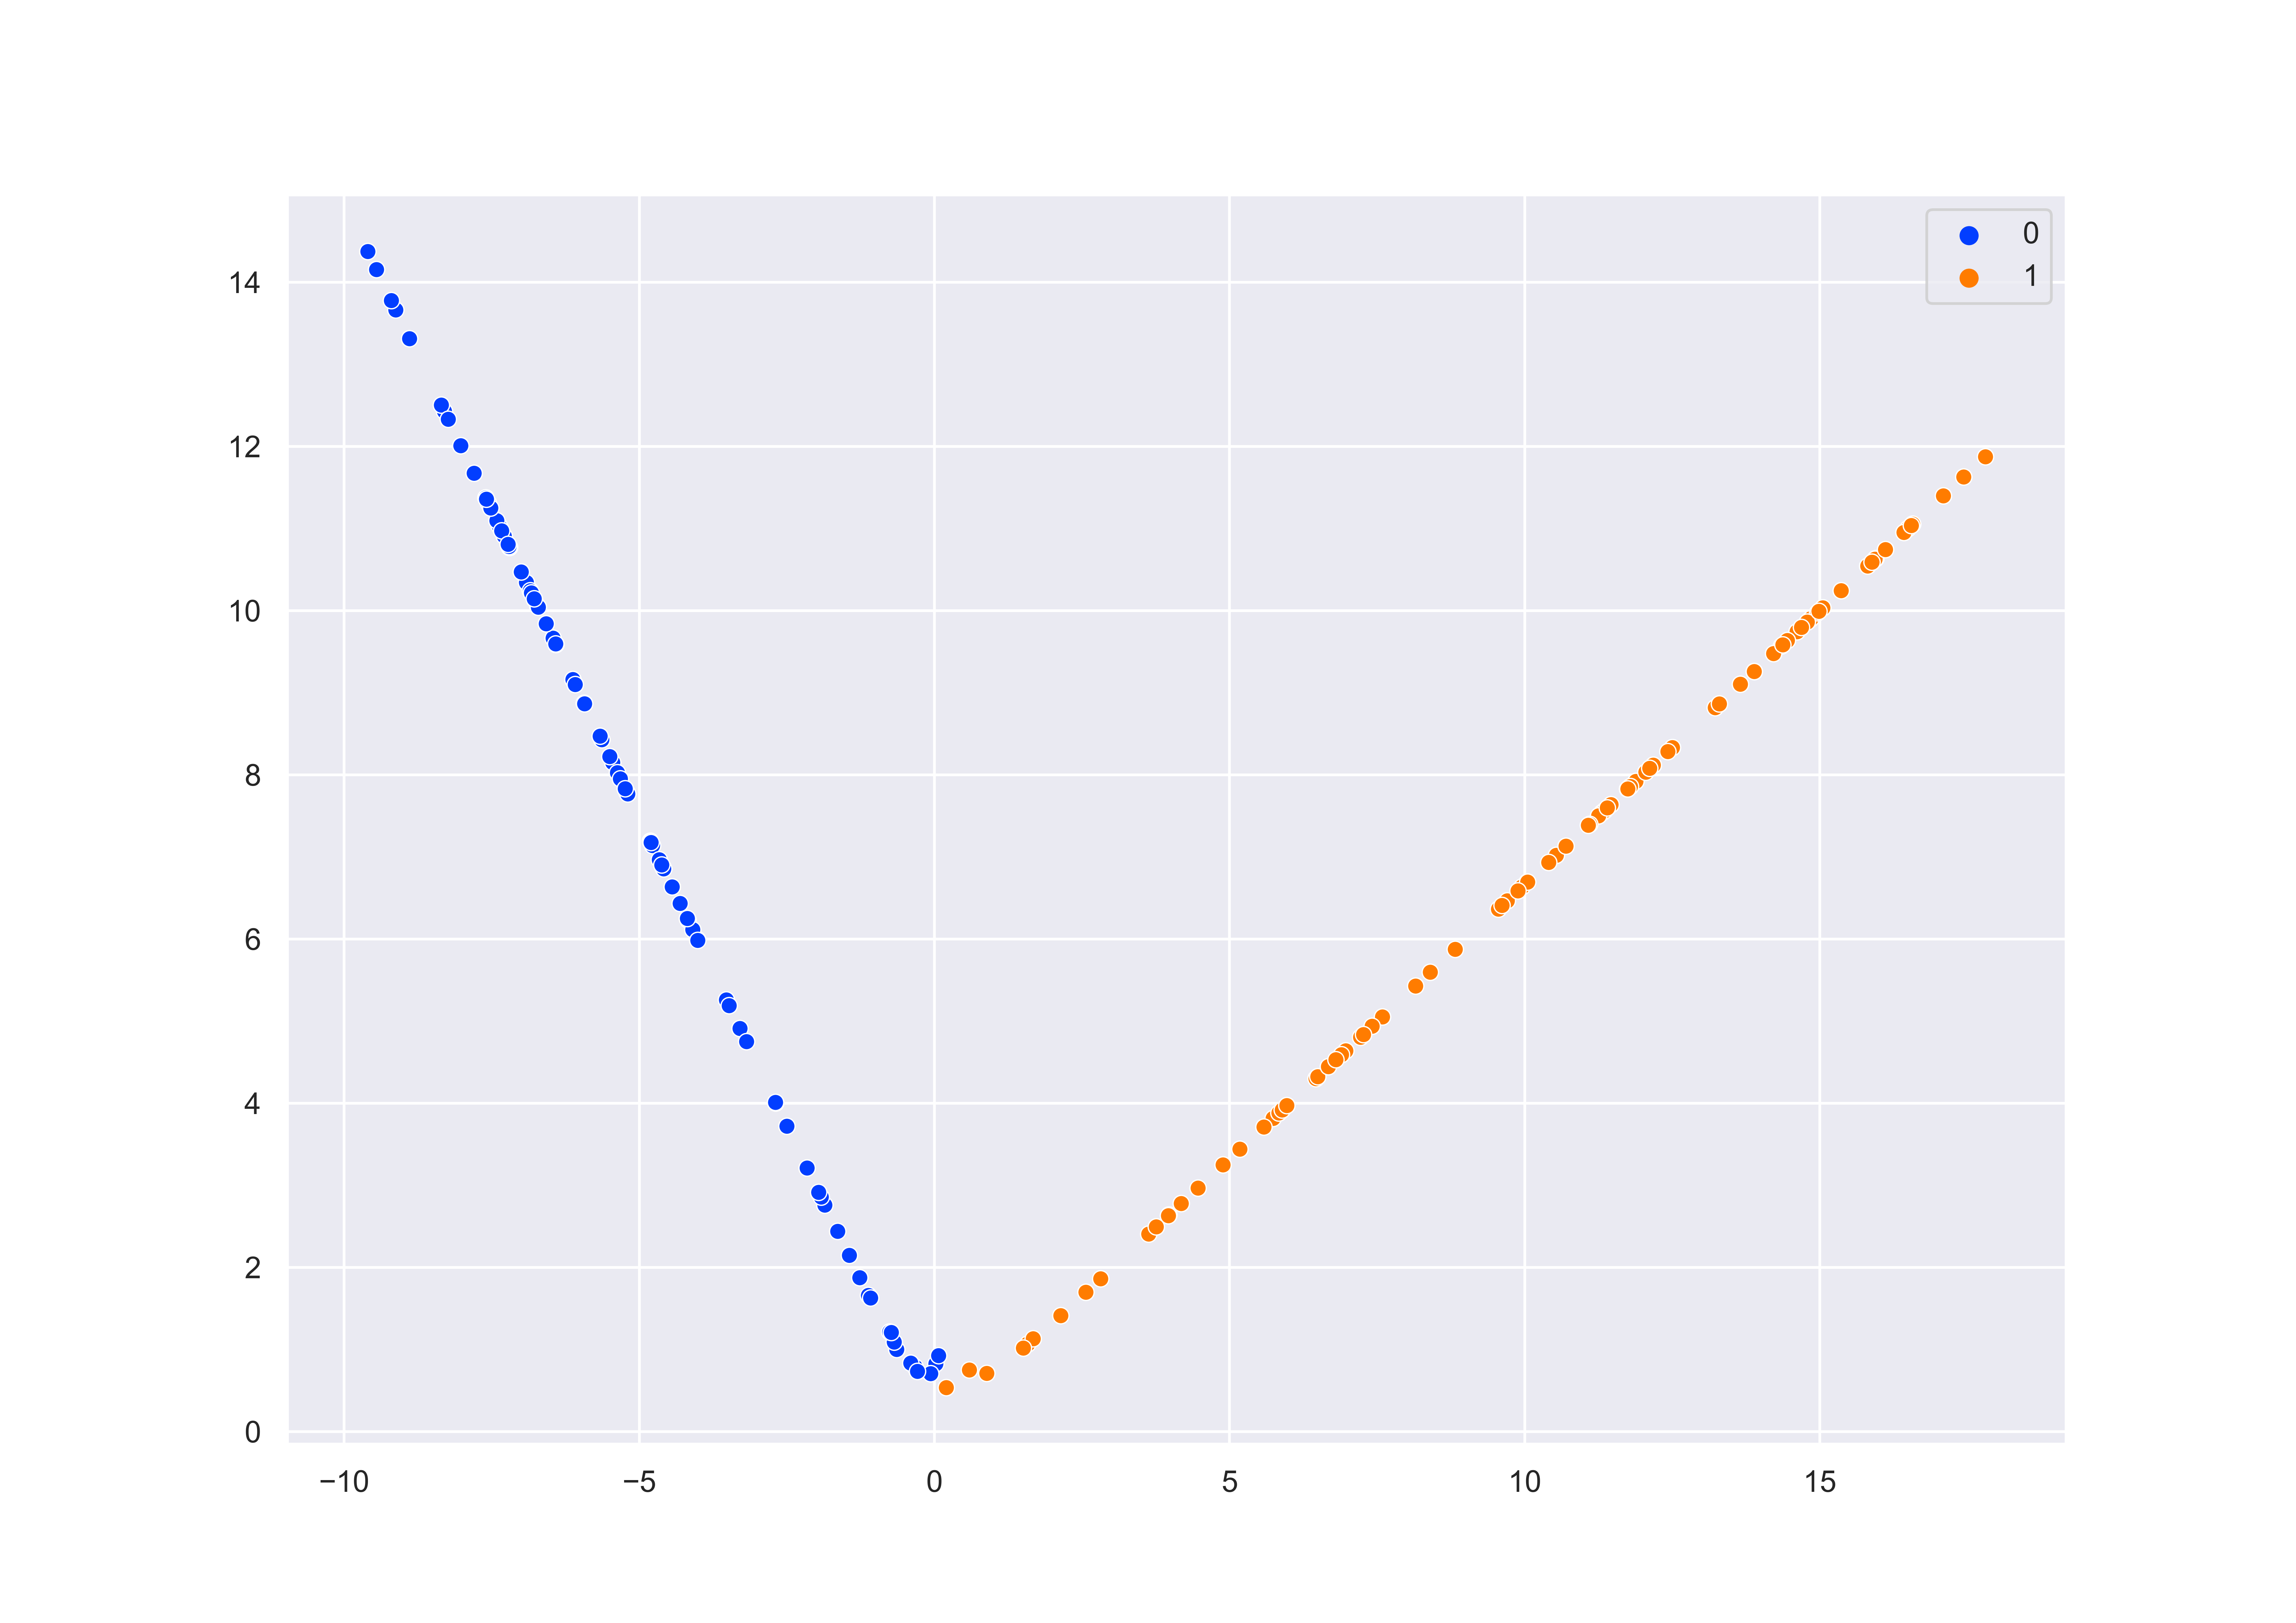
\includegraphics[width=0.45\linewidth]{../images/sst2_feature_map4_pca.png}
        % \caption{Absolute value of indivisual components of weight in ridge regression when setting $\lambda$ to 1.5.}
        % \label{fig:mnist_tSNE_3}
    \end{subfigure}
    \caption{Visualization images of intermediate output tensors with PCA method. Top-Left: Tensors after the first LSTM layer. Top-Right: Tensors after the second LSTM layer. Bottom-Left: Tensors after the final LSTM layer. Bottom-Right: Tensors after the first linear layer.}
    \label{fig:sst_pca}
\end{figure}

\begin{figure}[htbp]
    \centering
    \begin{subfigure}
        \centering
        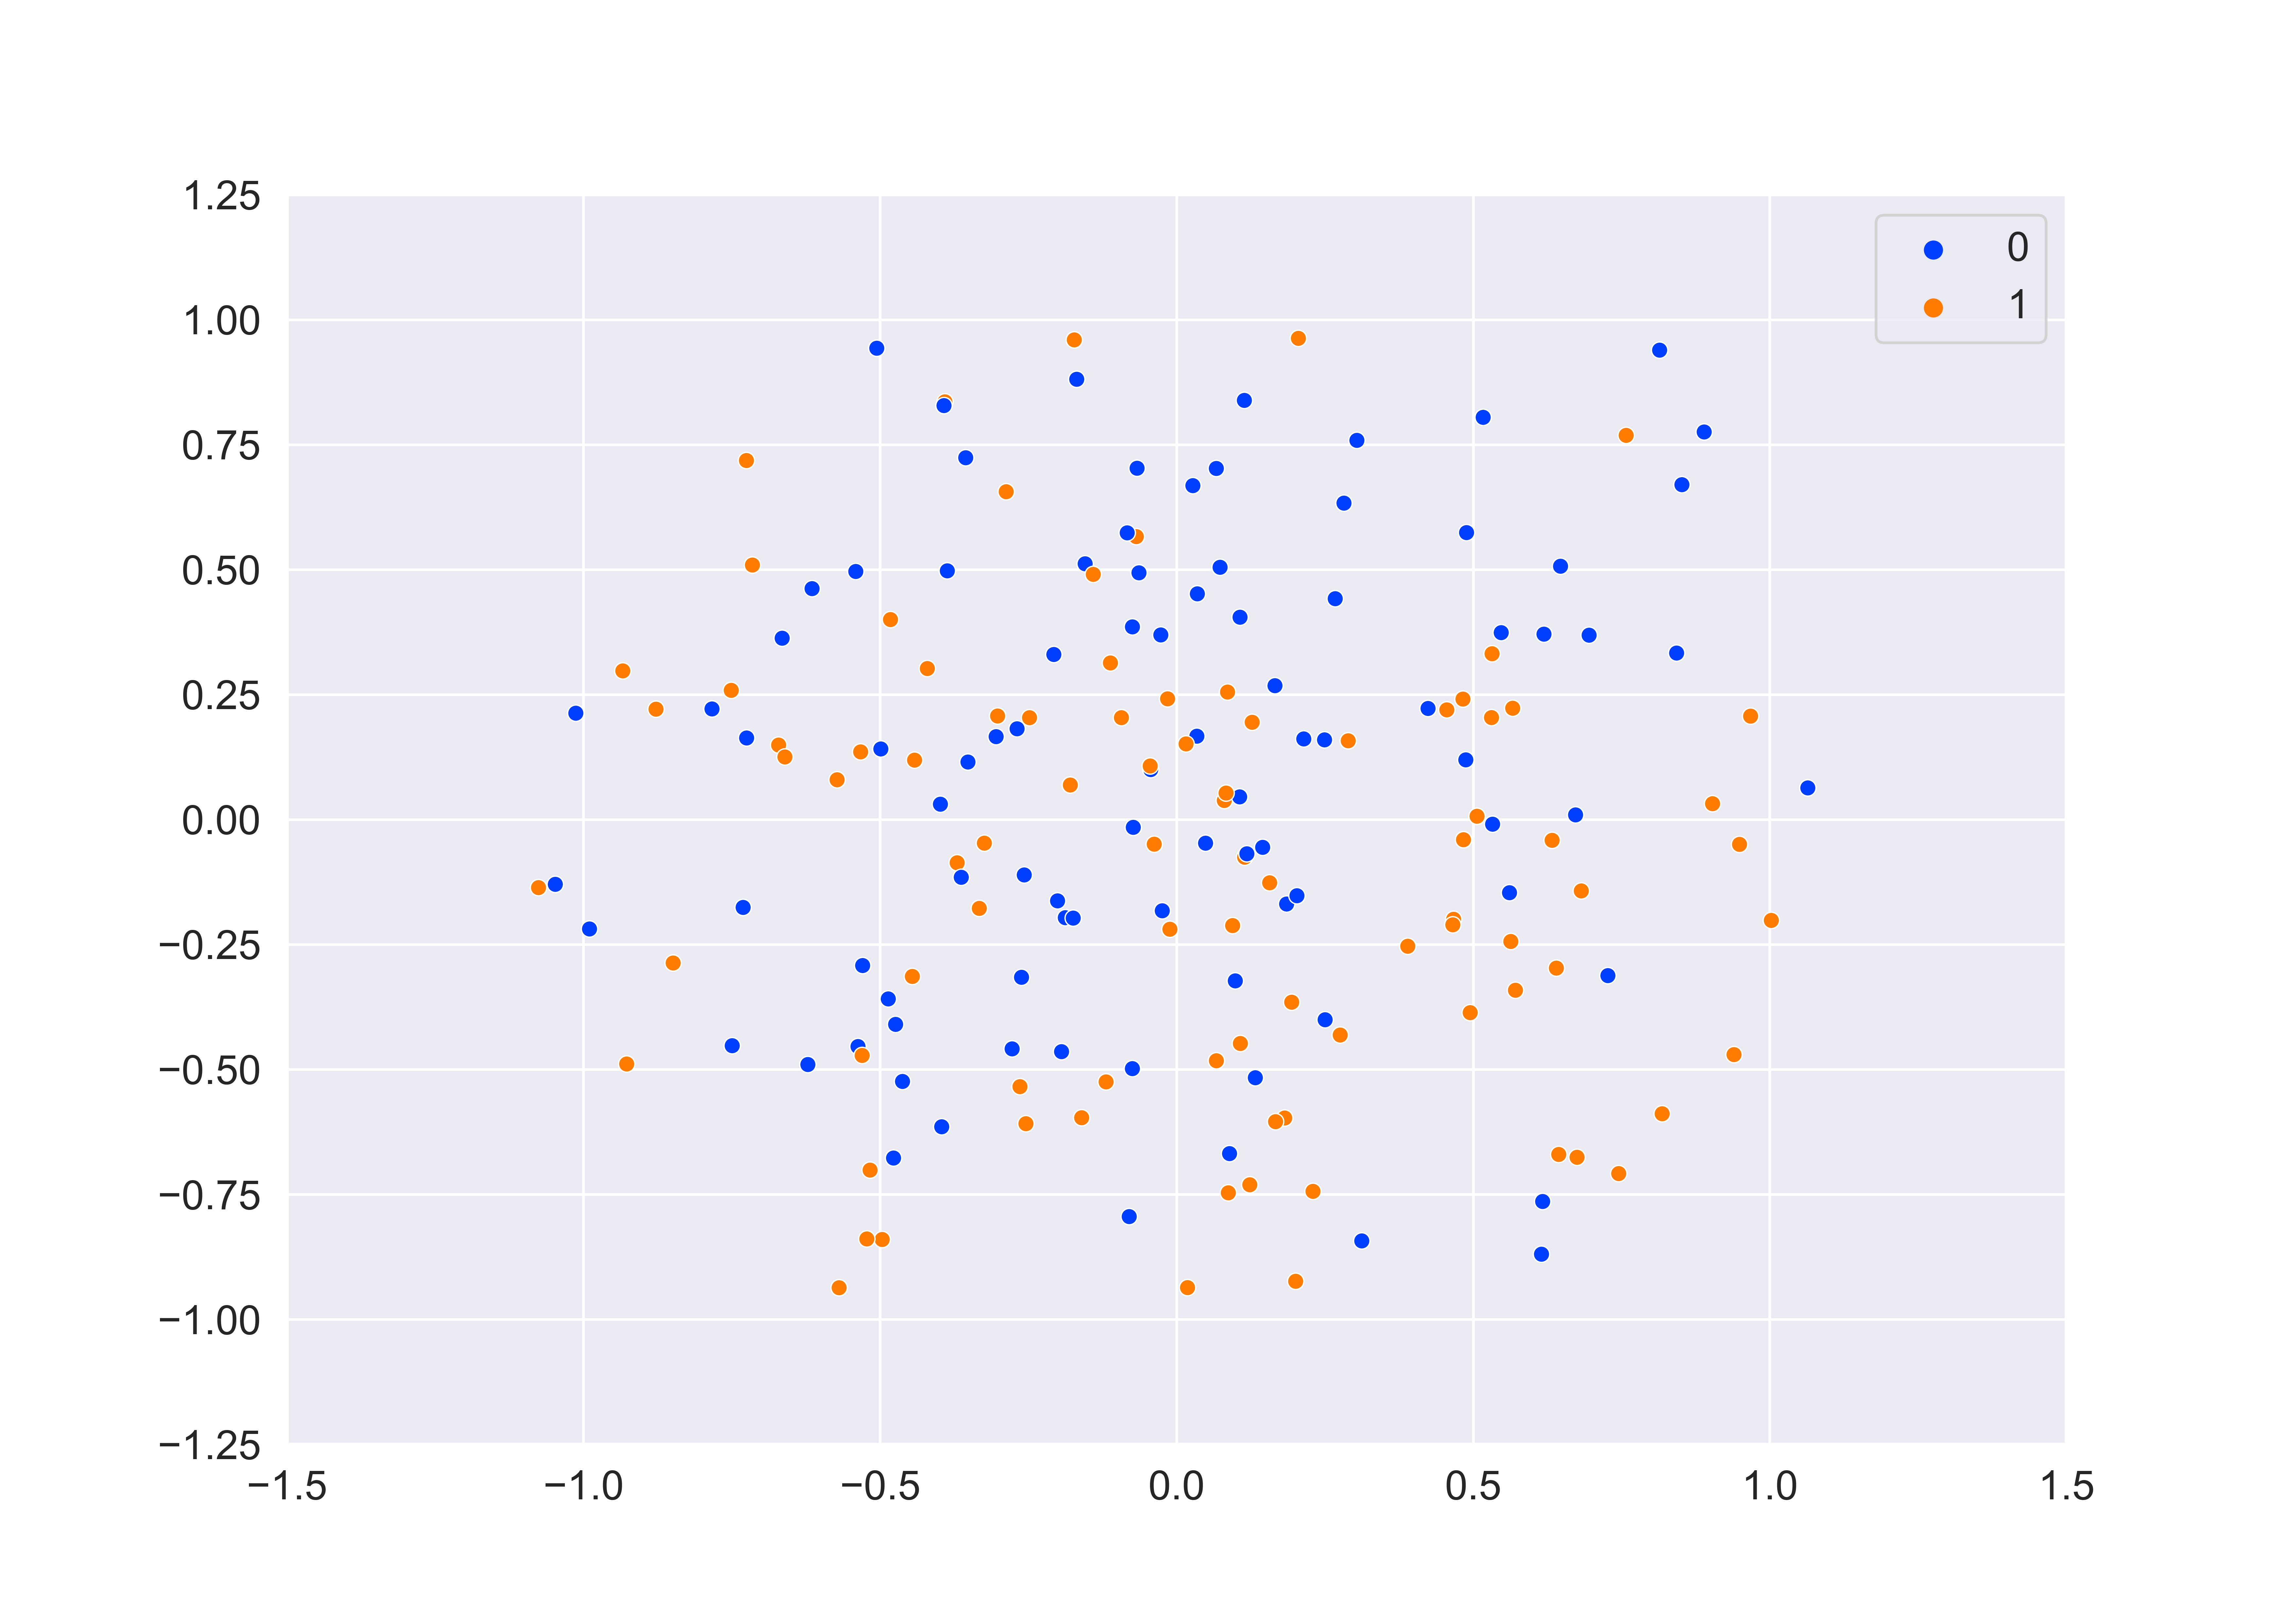
\includegraphics[width=0.45\linewidth]{../images/sst2_feature_map1_tsne.png}
        % \caption{a}
        % \label{fig:mnist_tSNE_1}
    \end{subfigure}
    % \hfill 
    \begin{subfigure}
        \centering
        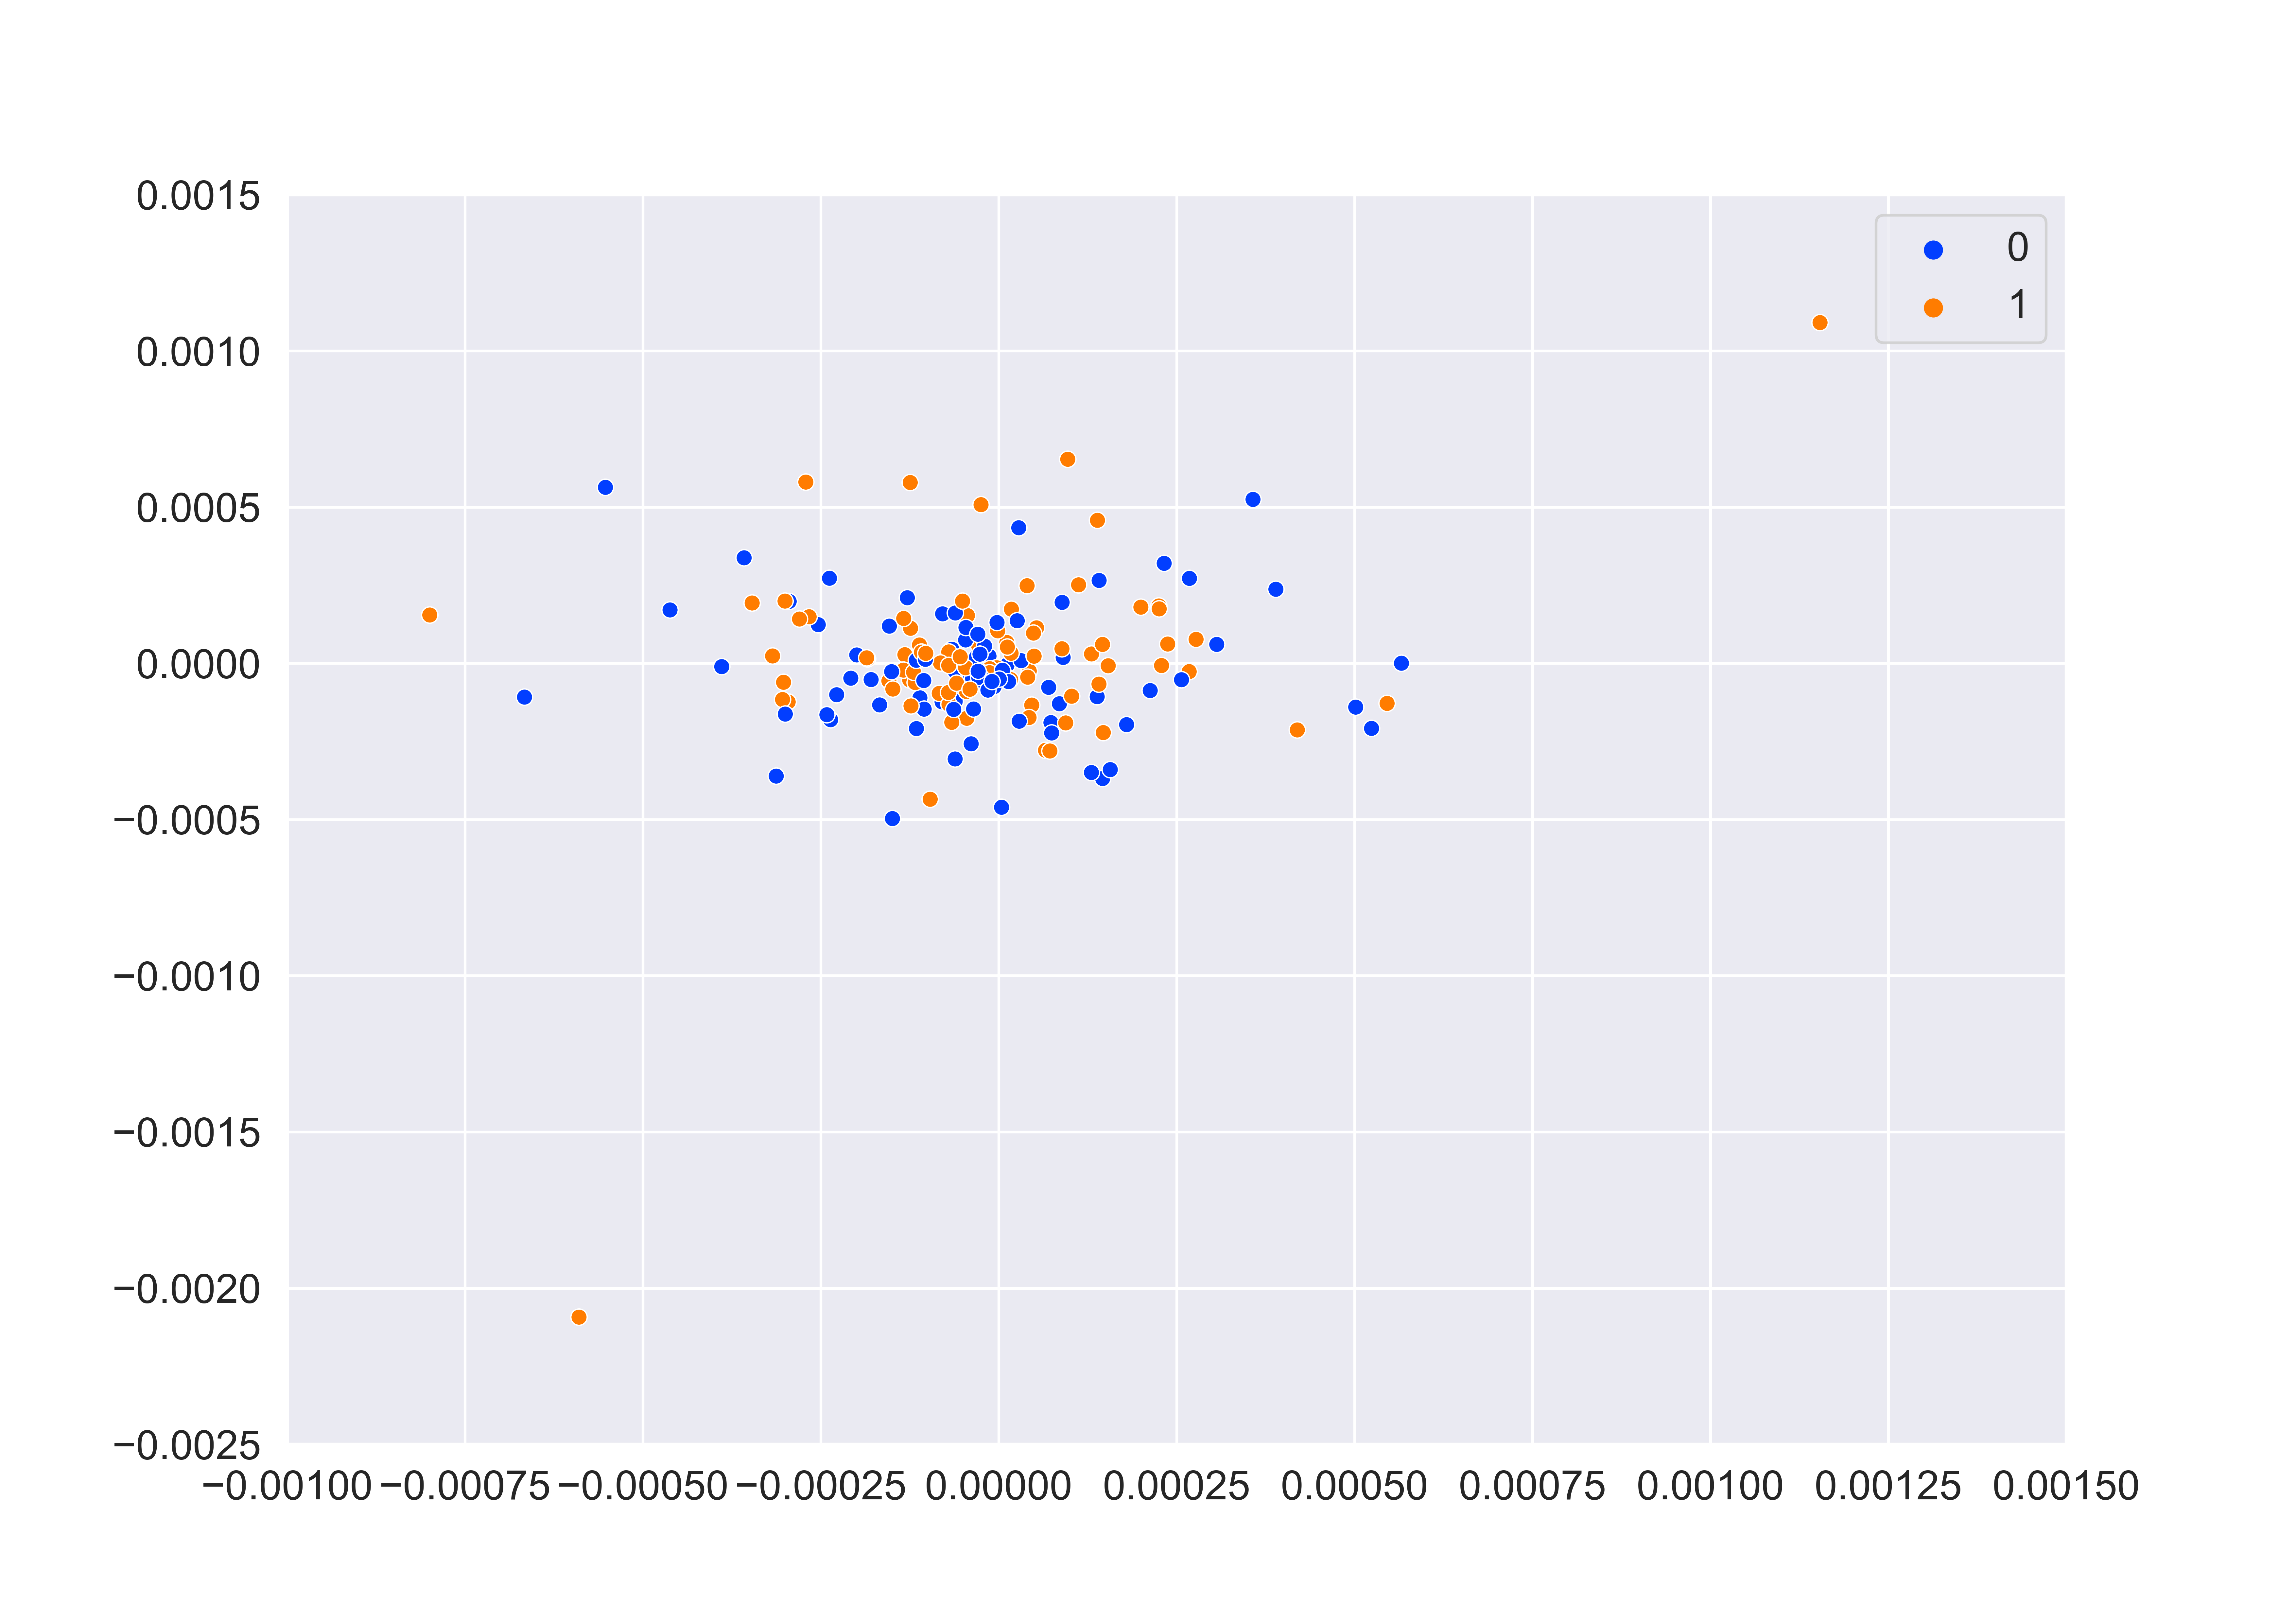
\includegraphics[width=0.45\linewidth]{../images/sst2_feature_map2_tsne.png}
        % \caption{Absolute value of indivisual components of weight in ridge regression when setting $\lambda$ to 1.0.}
        % \label{fig:mnist_tSNE_2}
    \end{subfigure}
    % \hfill 
    \begin{subfigure}
        \centering
        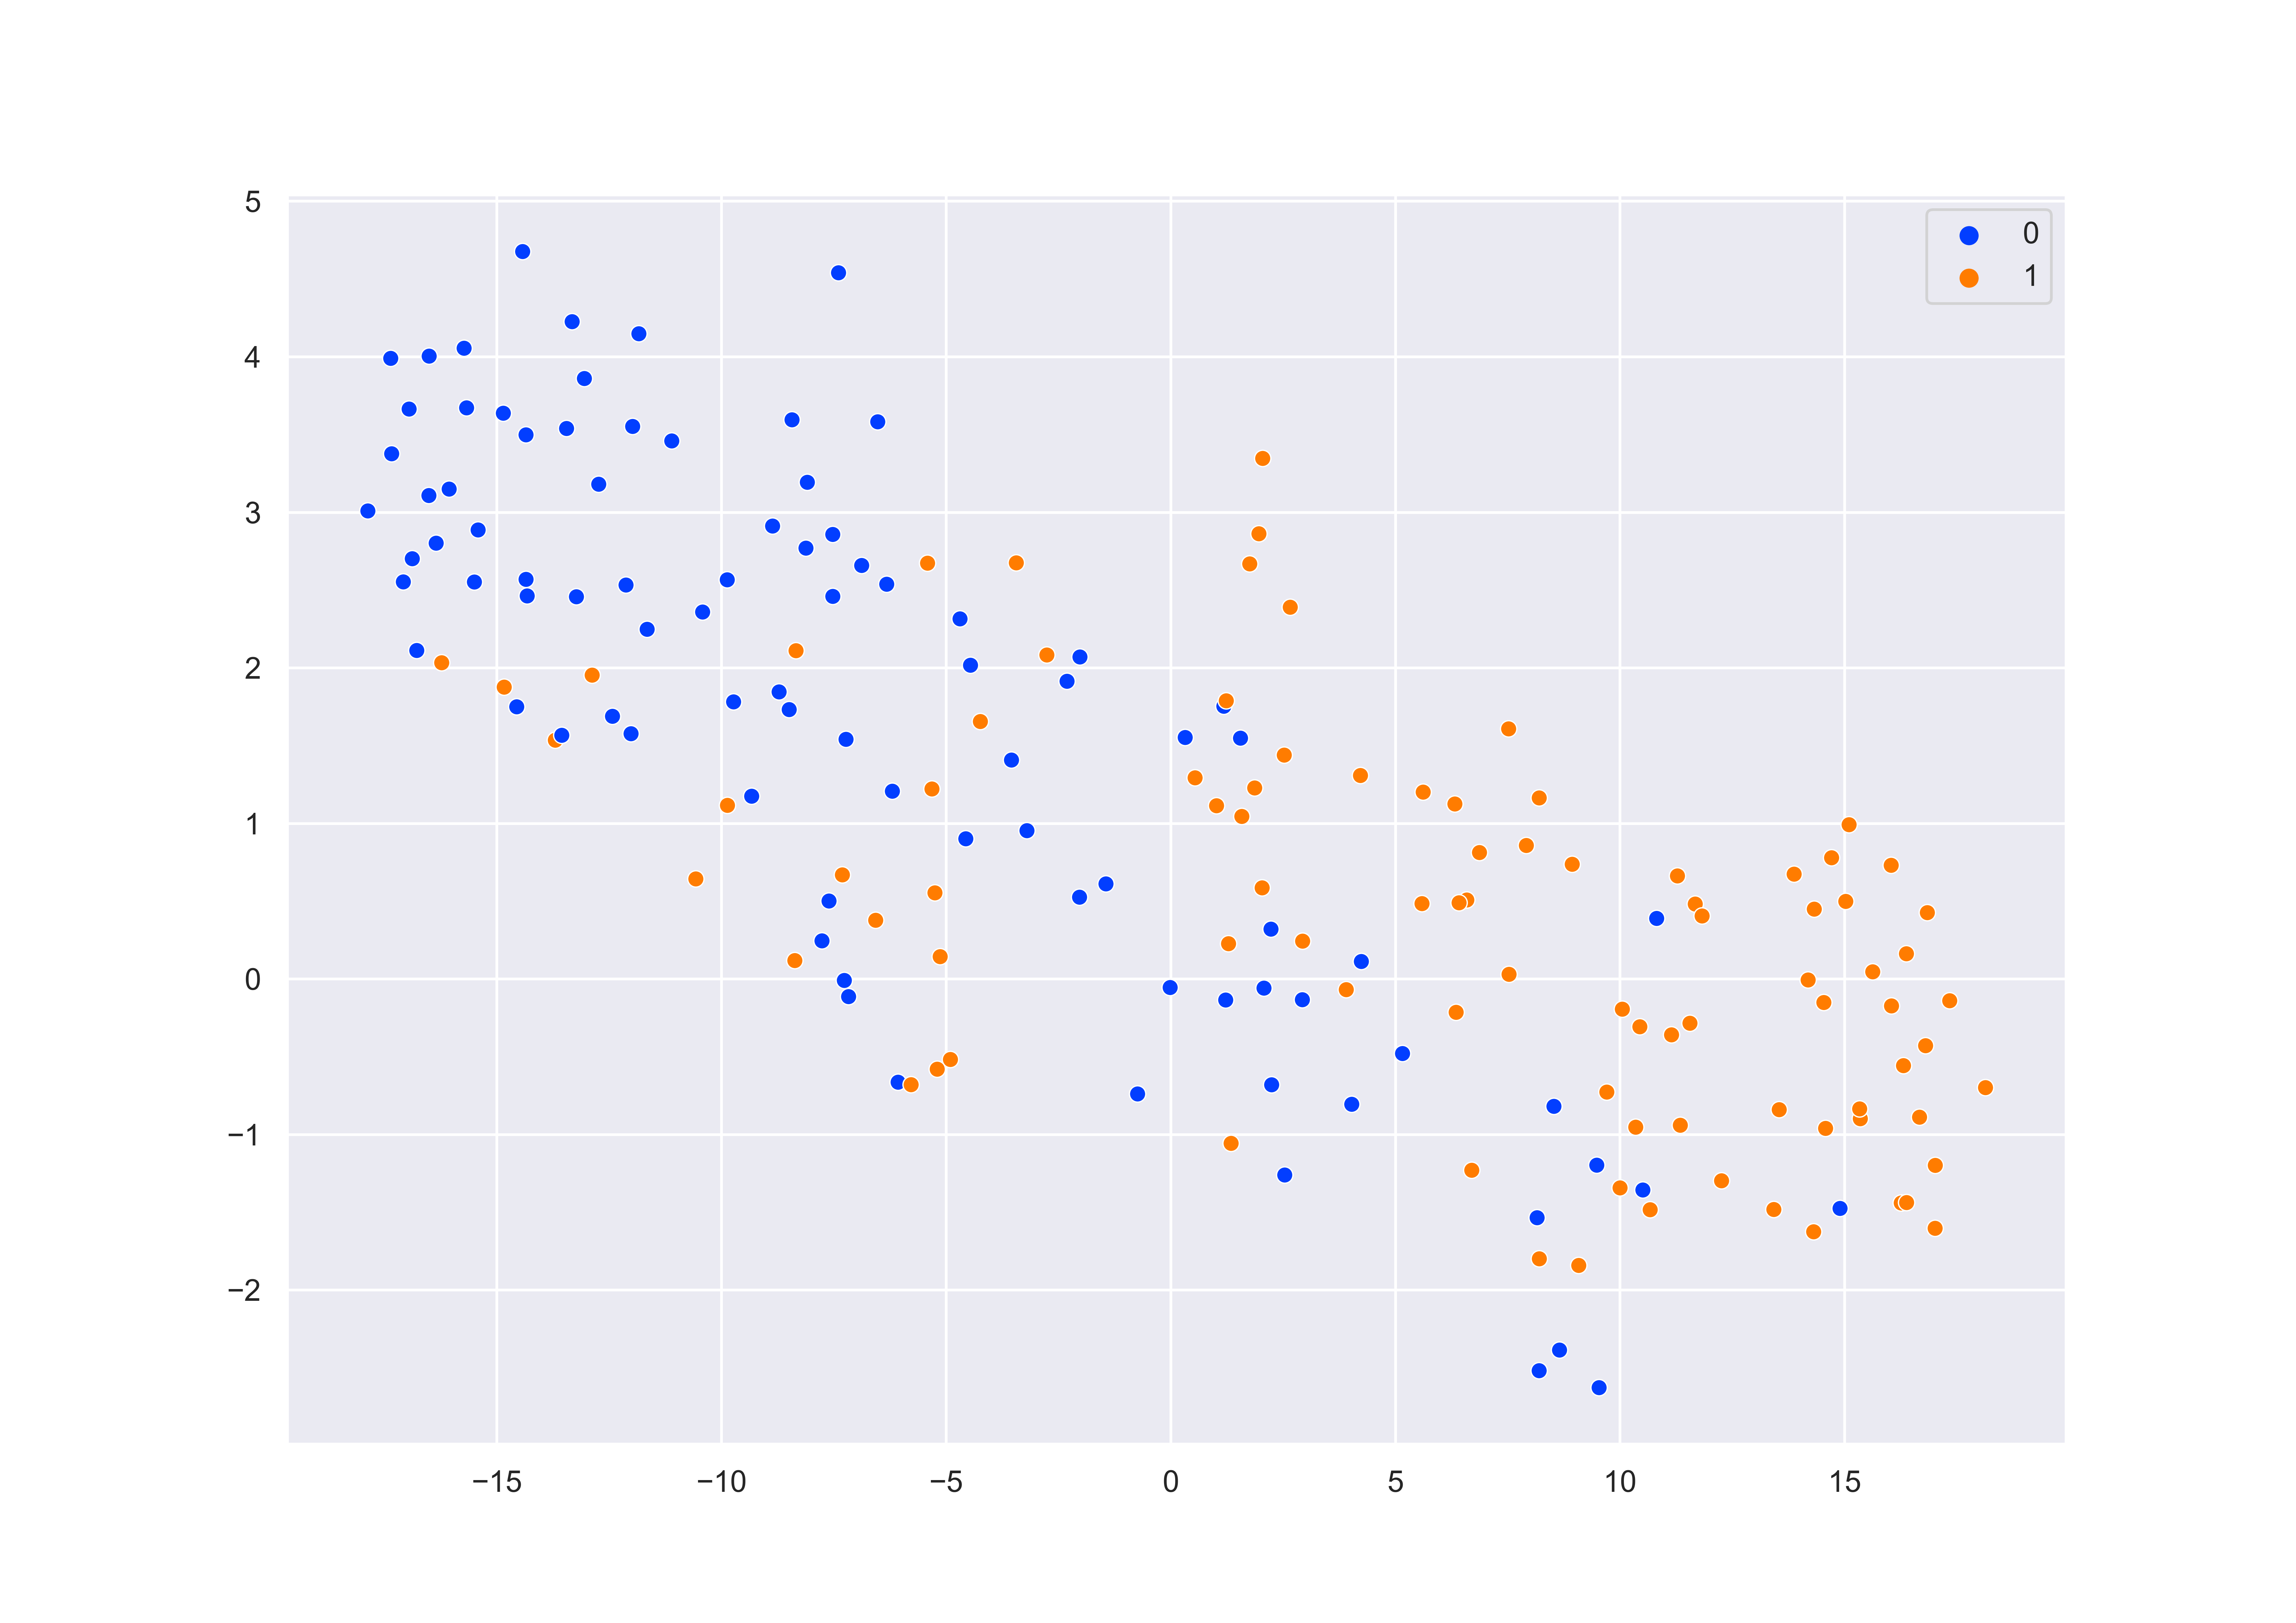
\includegraphics[width=0.45\linewidth]{../images/sst2_feature_map3_tsne.png}
        % \caption{Absolute value of indivisual components of weight in ridge regression when setting $\lambda$ to 1.5.}
        % \label{fig:mnist_tSNE_3}
    \end{subfigure}
    \begin{subfigure}
        \centering
        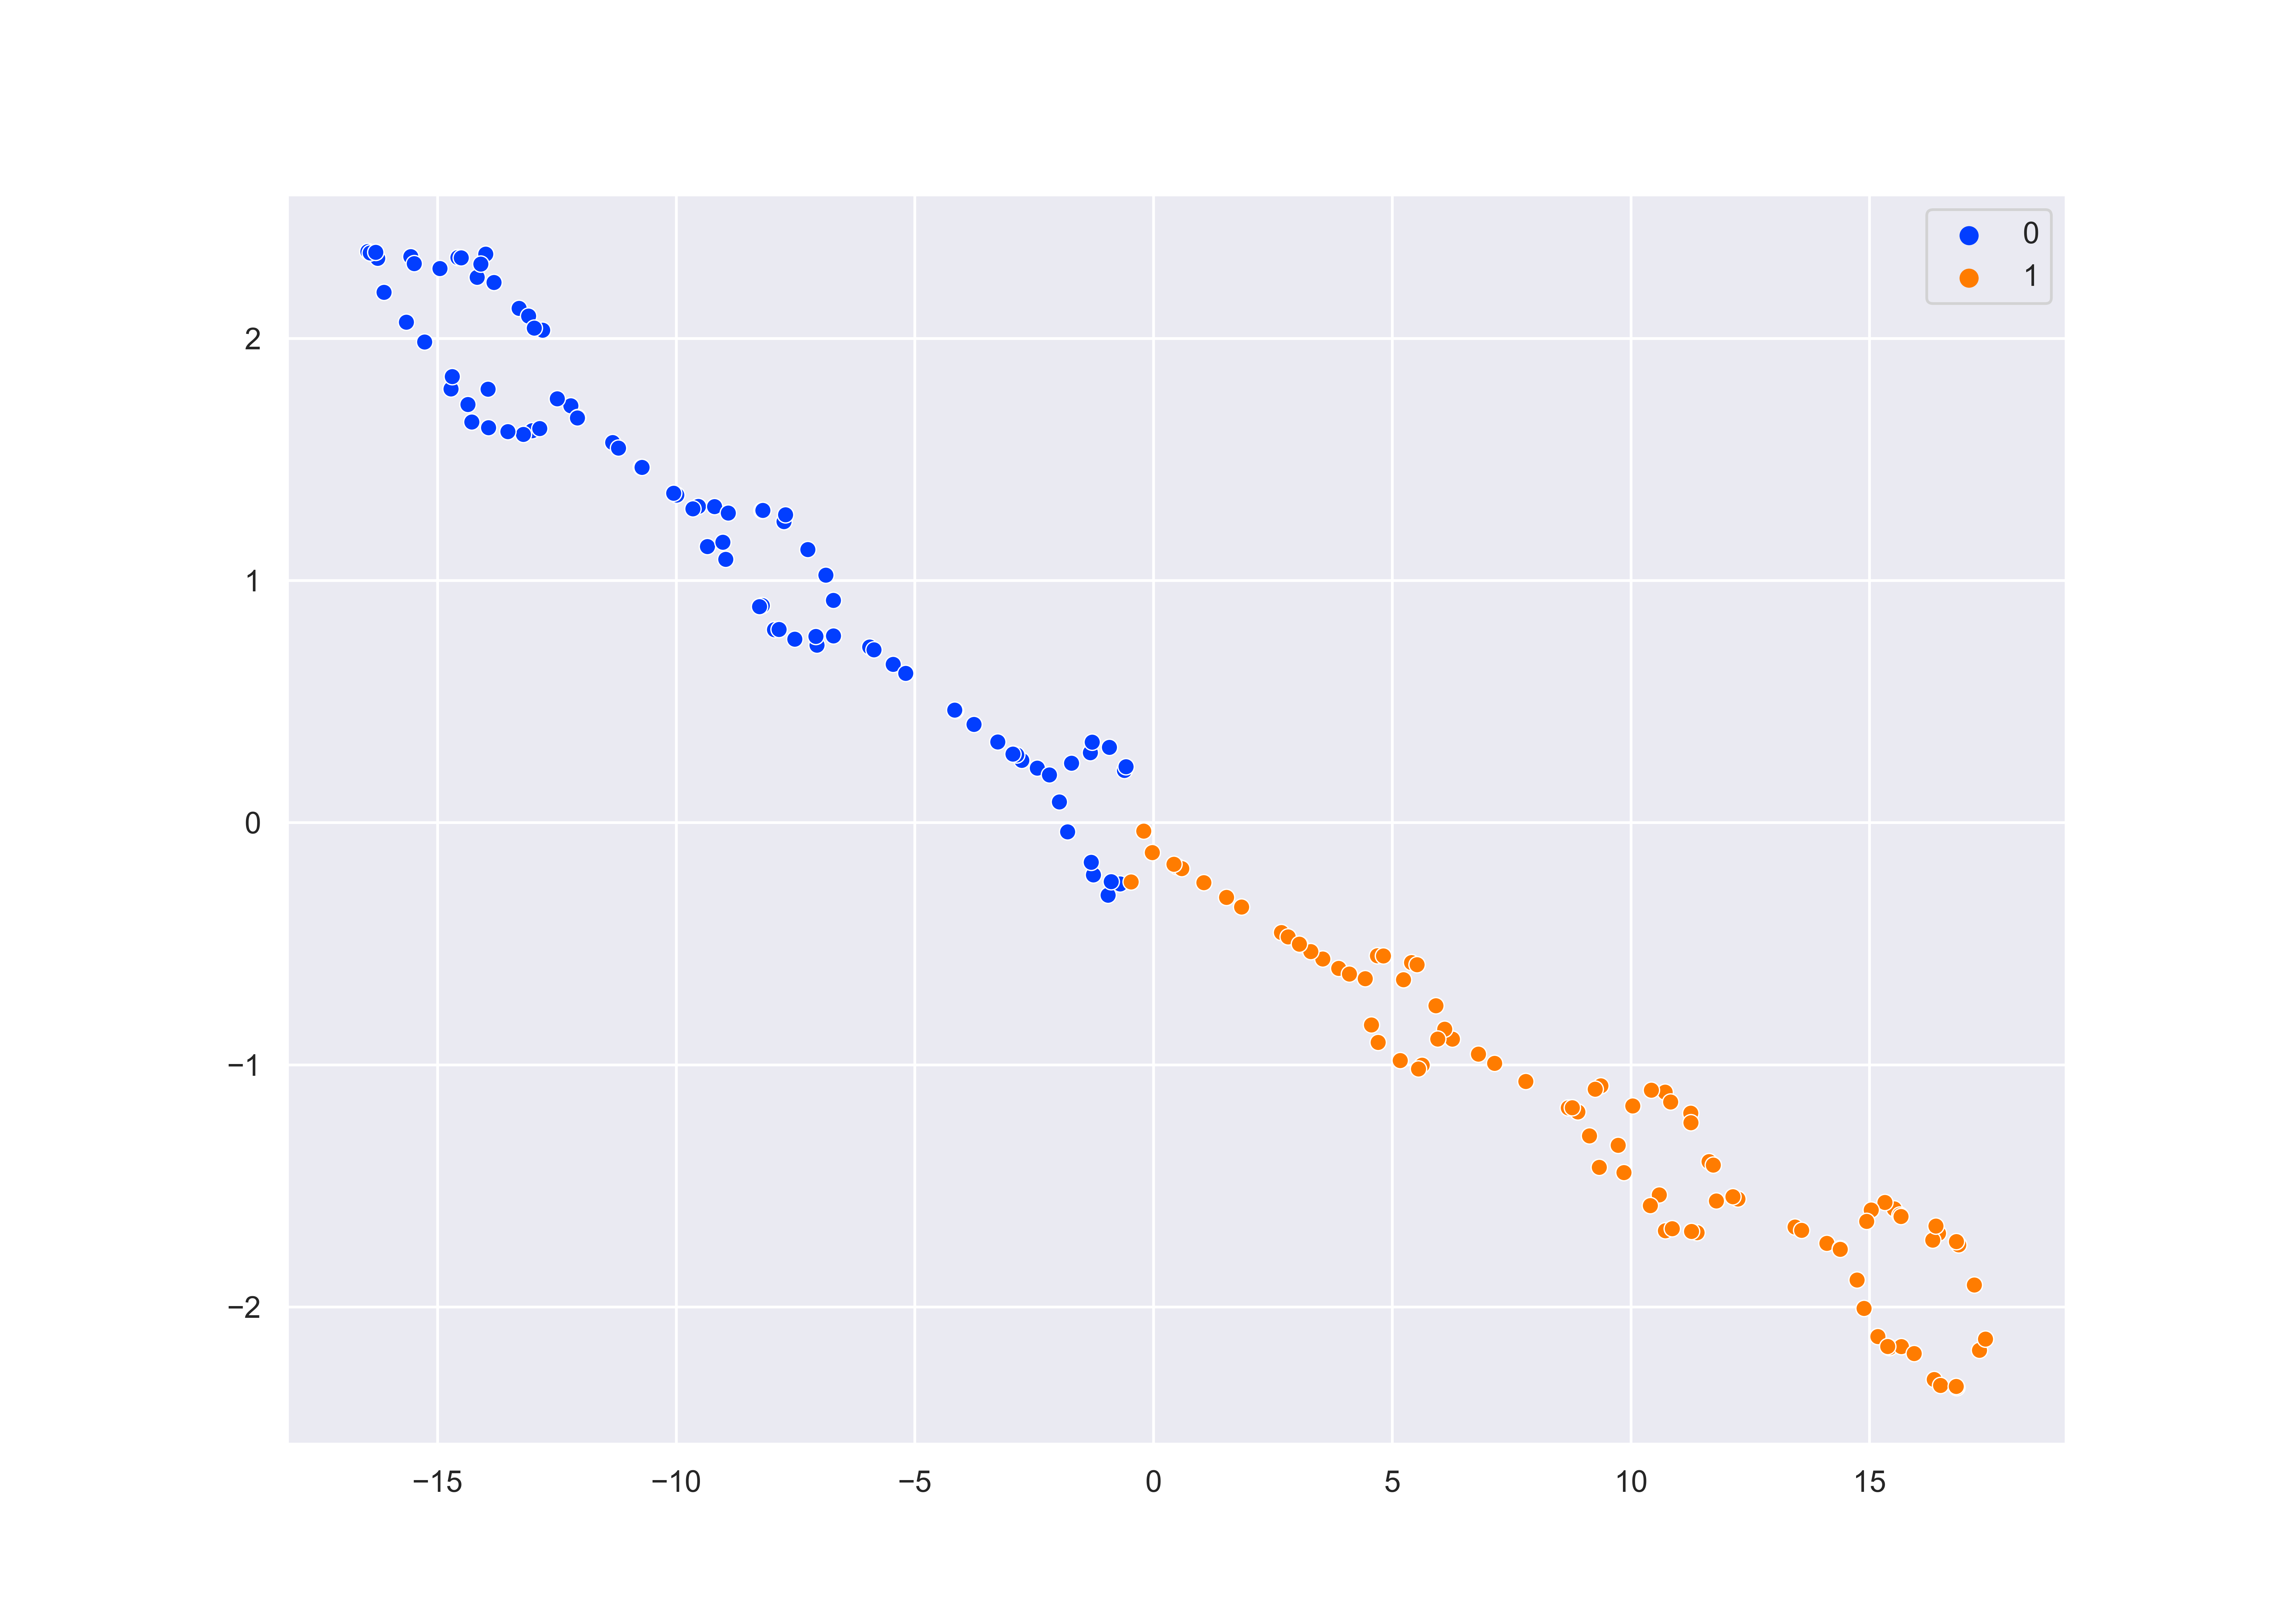
\includegraphics[width=0.45\linewidth]{../images/sst2_feature_map4_tsne.png}
        % \caption{Absolute value of indivisual components of weight in ridge regression when setting $\lambda$ to 1.5.}
        % \label{fig:mnist_tSNE_3}
    \end{subfigure}
    \caption{Visualization images of intermediate output tensors with t-SNE method. Top-Left: Tensors after the first LSTM layer. Top-Right: Tensors after the second LSTM layer. Bottom-Left: Tensors after the final LSTM layer. Bottom-Right: Tensors after the first linear layer.}
    \label{fig:sst_tsne}
\end{figure}

\subsection{Loss Function}
Again, in classification setting, I again add an additional logarithm operation after softmax function for stable computation. 
And I again use negative log-liklihood function defined in Eq.~\ref{eq:nllloss}, where $K=2$ in this setting.

\subsection{Experiment Result}
The training accuracy and validation accuracy are plotted in Fig.~\ref{fig:sst-train_loss} and Fig.~\ref{fig:sst-dev_loss}. 
The best checkpoint can achieve $70.52\%$ accuracy, which is on par with fine-trained LSTM models.
From training loss figure, the loss is smoothly decreasing, meaning that the learning rate is appropriate.
From validation loss figure, the validation loss is increasing but accuracy is also increasing in the first 10 epochs. 
After 10 epochs, the validation accuracy is fluctuating between $70\%$ and $72\%$.
So it verifies that if I need to tune the hyperparameters, I can lower down the learning rate after 10 epochs for better result.
But I do not choose to do so because tuning hyperparamters costs computational resources a lot and is meaningless in this task.
\newline
\newline
\noindent 
Besides, I sample the last token of each sentence after each LSTM layers and the tensor after the first linear layer for visualization.
Their corresponding visualization result is presented in Fig.~\ref{fig:sst_pca} with PCA method and Fig.~\ref{fig:sst_tsne} with t-SNE method, respectively.
It can be seen that at the beginning of the LSTM layers, my model cannot well distinguish the negative samples and positive samples well.
But after the final LSTM layer and the first linear layer, the datapoint can be separated well by my model, which again verifies the correctness of my LSTM model.

\subsection{Discussion}
The accuracy can be improved from two aspects. First, use pretrained word embedding for each word, such as word2vec or Bert-initialized word embedding. 
These word embeddings can assign more semantic information for one specific word, including the word itself and its neighbors.
The hidden state of each word can be more representative and further enhance the accuracy.
\newline
\newline
\noindent 
Second, I only consider one way, that is left-to-right information, while to predict the sentiment of a sentence, the former word can also count.
Therefore, the accuracy can be improved by adopting BiLSTM instead of vanilla LSTM.
\newline
\newline
\noindent 
Apart from improvable points, the stacked layers of LSTM may not count a lot. 
Maybe a 2-layer LSTM model can also achieve the same accuracy with less computational cost. 
Increase of parameters only make a different when the input is not sophisticated enough.